\documentclass[9pt]{article}
\usepackage[english]{babel}
\usepackage{amsmath,amsthm}
\usepackage{amsfonts}
\usepackage{graphicx}
\usepackage[margin=0.2in]{geometry}
\newcommand{\setlinespacing}[1]{\setlength{\baselineskip}{#1 \defbaselineskip}}
\newcommand{\doublespacing}{\setlength{\baselineskip}{2.0 \defbaselineskip}}
\newcommand{\singlespacing}{\setlength{\baselineskip}{\defbaselineskip}}
\newcommand{\A}{{\cal A}}
\newcommand{\h}{{\cal H}}
\newcommand{\s}{{\cal S}}
\newcommand{\W}{{\cal W}}
\newcommand{\BH}{\mathbf B(\cal H)}
\newcommand{\KH}{\cal  K(\cal H)}
\newcommand{\Real}{\mathbb R}
\newcommand{\Complex}{\mathbb C}
\newcommand{\Field}{\mathbb F}
\newcommand{\RPlus}{[0,\infty)}
\newcommand{\norm}[1]{\left\Vert#1\right\Vert}
\newcommand{\essnorm}[1]{\norm{#1}_{\text{\rm\normalshape ess}}}
\newcommand{\abs}[1]{\left\vert#1\right\vert}
\newcommand{\set}[1]{\left\{#1\right\}}
\newcommand{\seq}[1]{\left<#1\right>}
\newcommand{\eps}{\varepsilon}
\newcommand{\To}{\longrightarrow}
\newcommand{\RE}{\operatorname{Re}}
\newcommand{\IM}{\operatorname{Im}}
\newcommand{\Poly}{{\cal{P}}(E)}
\newcommand{\EssD}{{\cal{D}}}
\newcommand{\field}[1]{\mathbb{#1}}
\newcommand{\C}{\field{C}}
\newcommand{\R}{\field{R}}
\newcommand{\script}[1]{\mathcal{#1}}
\newcommand{\fall}{\; \forall \;}
\newcommand{\exts}{\; \exists \;}
\newcommand{\mbf}[1]{\mathbf{#1}}
\newcommand{\binomial}[2]{\biggl( \begin{array}{c}  #1 \\ #2  \\ \end{array} \biggr) }
\newcommand{\fderiv}[2]{ \frac{d}{ d #1} \: #2}
\newcommand{\sderiv}[2]{ \frac{d^2}{ d^2 #1} \: #2}
\newcommand{\pfderiv}[2]{ \frac{\partial}{ \partial #1} \: #2}
\newcommand{\psderiv}[2]{ \frac{\partial^2}{ \partial^2 #1} \: #2}
\newcommand{\mat}[1]{\mathbf{#1}}
\DeclareSymbolFont{AMSb}{U}{msb}{m}{n}
\DeclareMathSymbol{\dblz}{\mathalpha}{AMSb}{"5A}
\DeclareMathSymbol{\dblr}{\mathalpha}{AMSb}{"52}
\DeclareMathSymbol{\dblt}{\mathalpha}{AMSb}{"54}
\DeclareMathSymbol{\dblq}{\mathalpha}{AMSb}{"51}
\DeclareMathSymbol{\dbln}{\mathalpha}{AMSb}{"4E}
\DeclareMathSymbol{\dblf}{\mathalpha}{AMSb}{"46}
\DeclareMathSymbol{\dblc}{\mathalpha}{AMSb}{"43}
\DeclareMathSymbol{\dbld}{\mathalpha}{AMSb}{"44}
\theoremstyle{plain}
\newtheorem{thm}{Theorem}[section]
\newtheorem{cor}[thm]{Corollary}
\newtheorem{lem}[thm]{Lemma}
\newtheorem{prop}[thm]{Proposition}
\theoremstyle{definition}
\newtheorem{defn}{Definition}[section]
\theoremstyle{remark}
\newtheorem{rem}{Remark}[section]
\numberwithin{equation}{section}
\renewcommand{\theequation}{\thesection.\arabic{equation}}
\begin{document}
\title{Regression of KL Software Distribution   }
\author{KL Software Libraries}
\date{Mon May 05 14:23:32 2014
}
\maketitle
\textbf{ KL Library test output.  This LaTex file and the associated diagrams are produced by the KL software libraries.}
\subsubsection{Matrix Quick Check <double>}
QueryPerformanceCounter  =  1.41172
\subsubsection{Matrix Quick Check <float>}
QueryPerformanceCounter  =  1.36498
\subsubsection{Intel VSL Function Check}
\includegraphics[width=10.0cm,height=10.0cm]{klVSLInv.pdf}

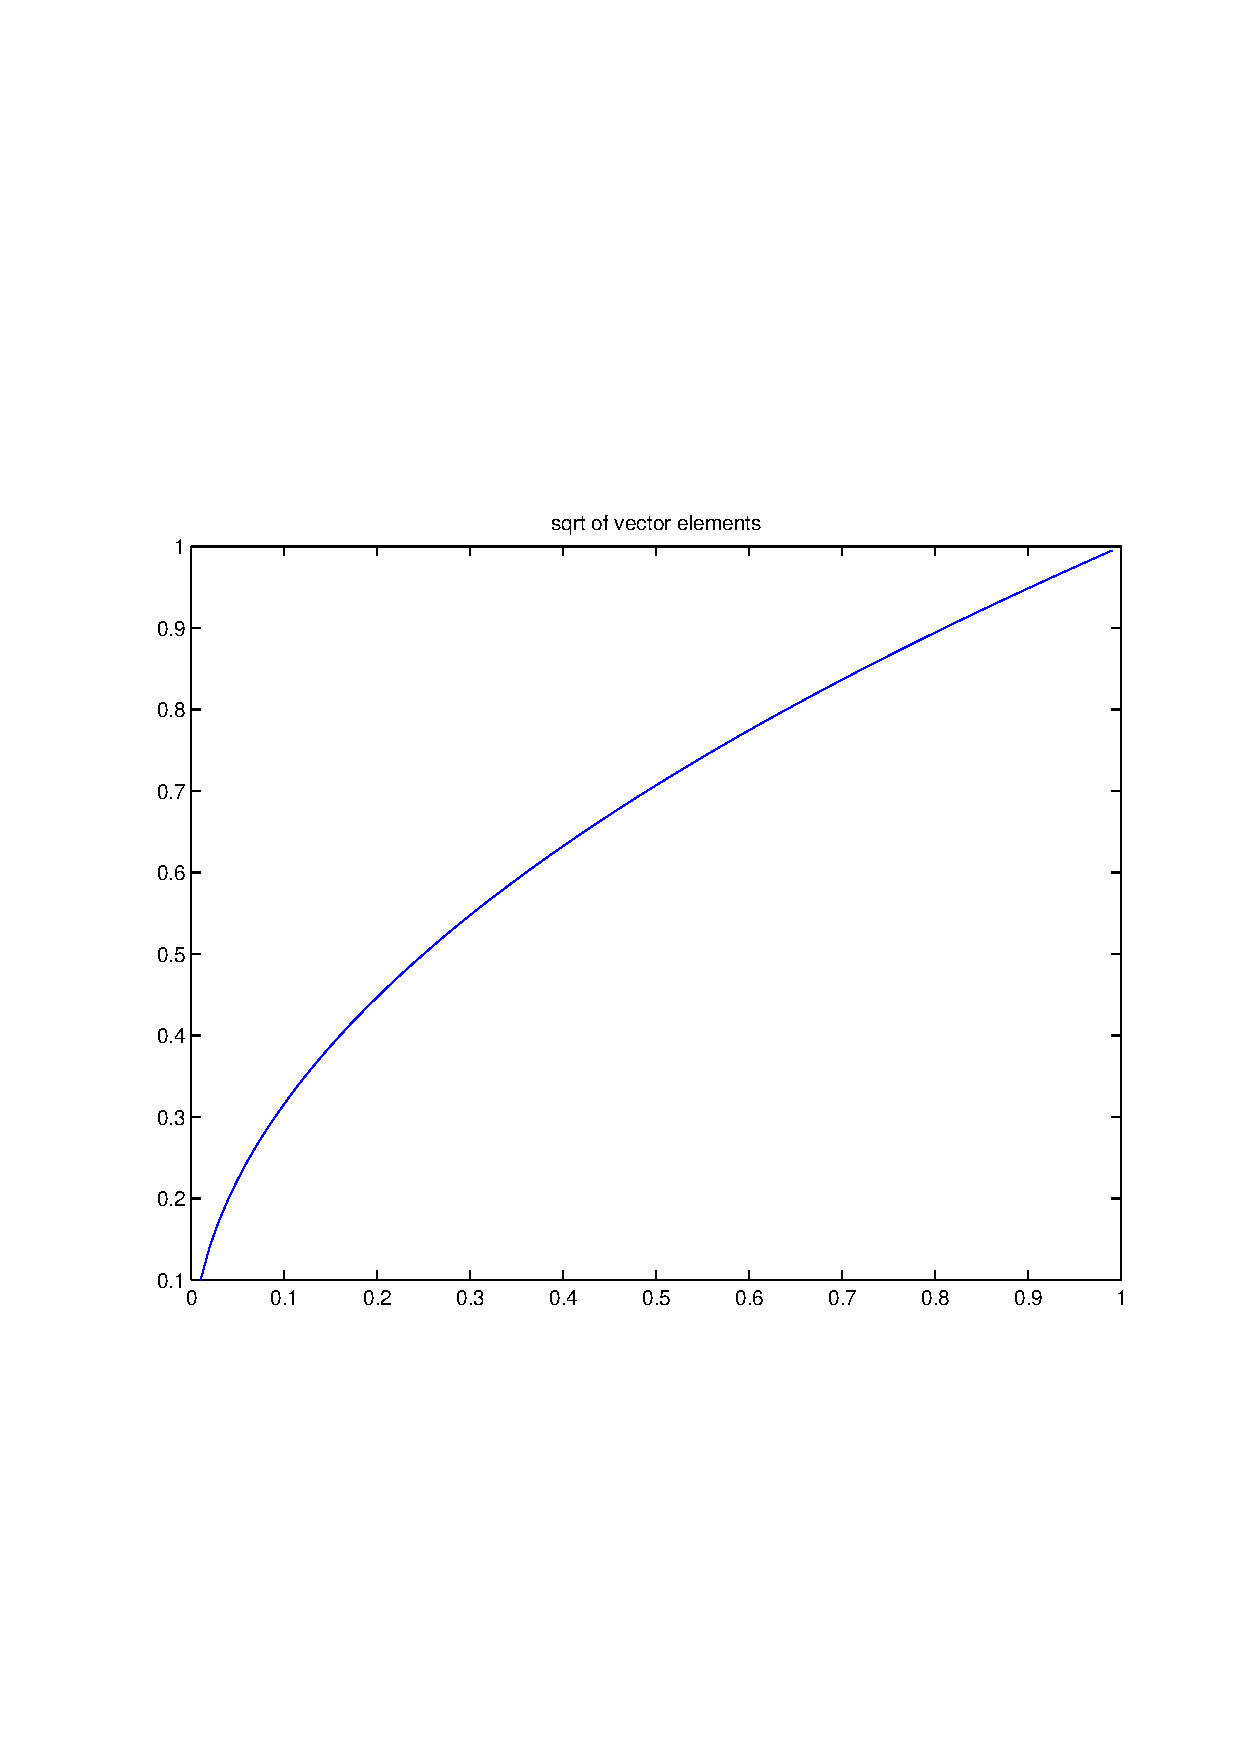
\includegraphics[width=10.0cm,height=10.0cm]{klVSLSqrt.pdf}

\includegraphics[width=10.0cm,height=10.0cm]{klVSLExp.pdf}

\includegraphics[width=10.0cm,height=10.0cm]{klVSLExpm1.pdf}

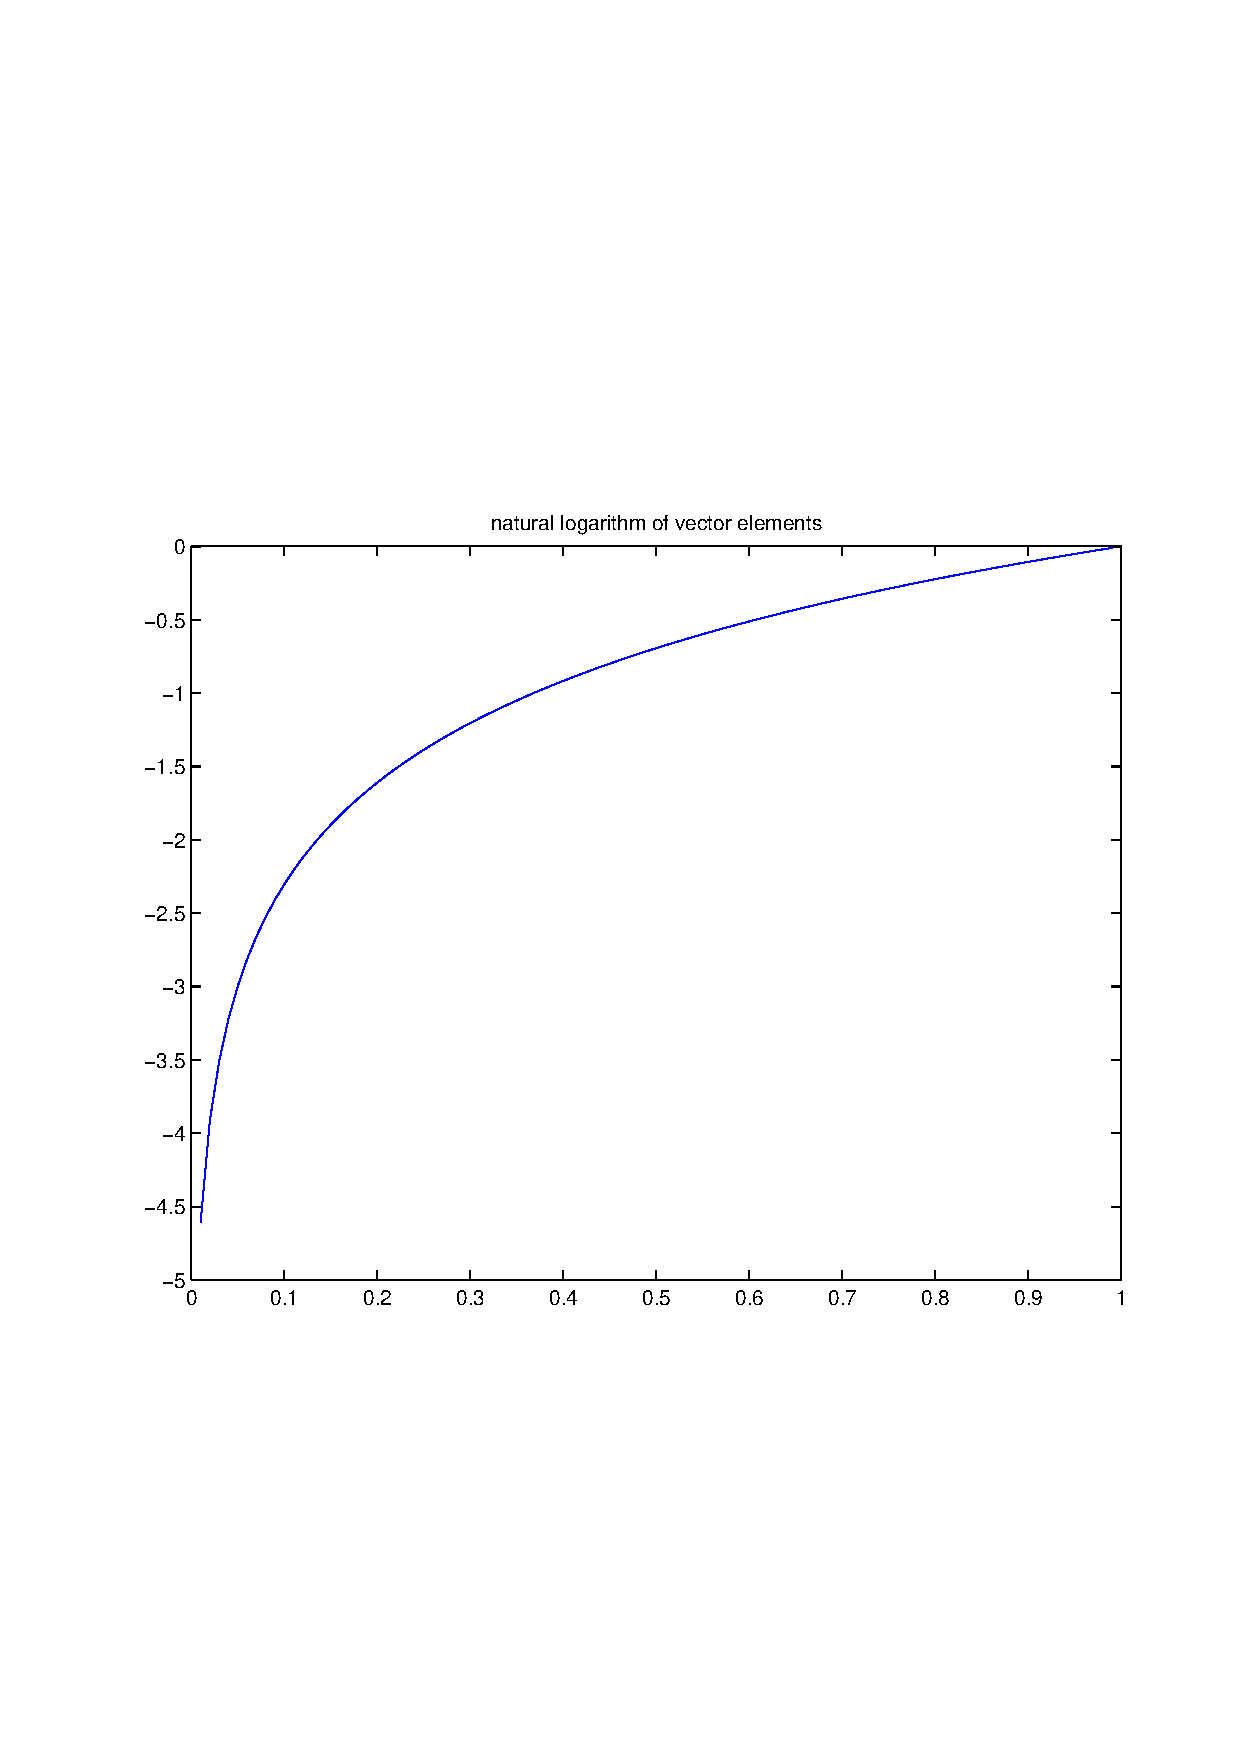
\includegraphics[width=10.0cm,height=10.0cm]{klVSLLn.pdf}

\includegraphics[width=10.0cm,height=10.0cm]{klVSLLog10.pdf}

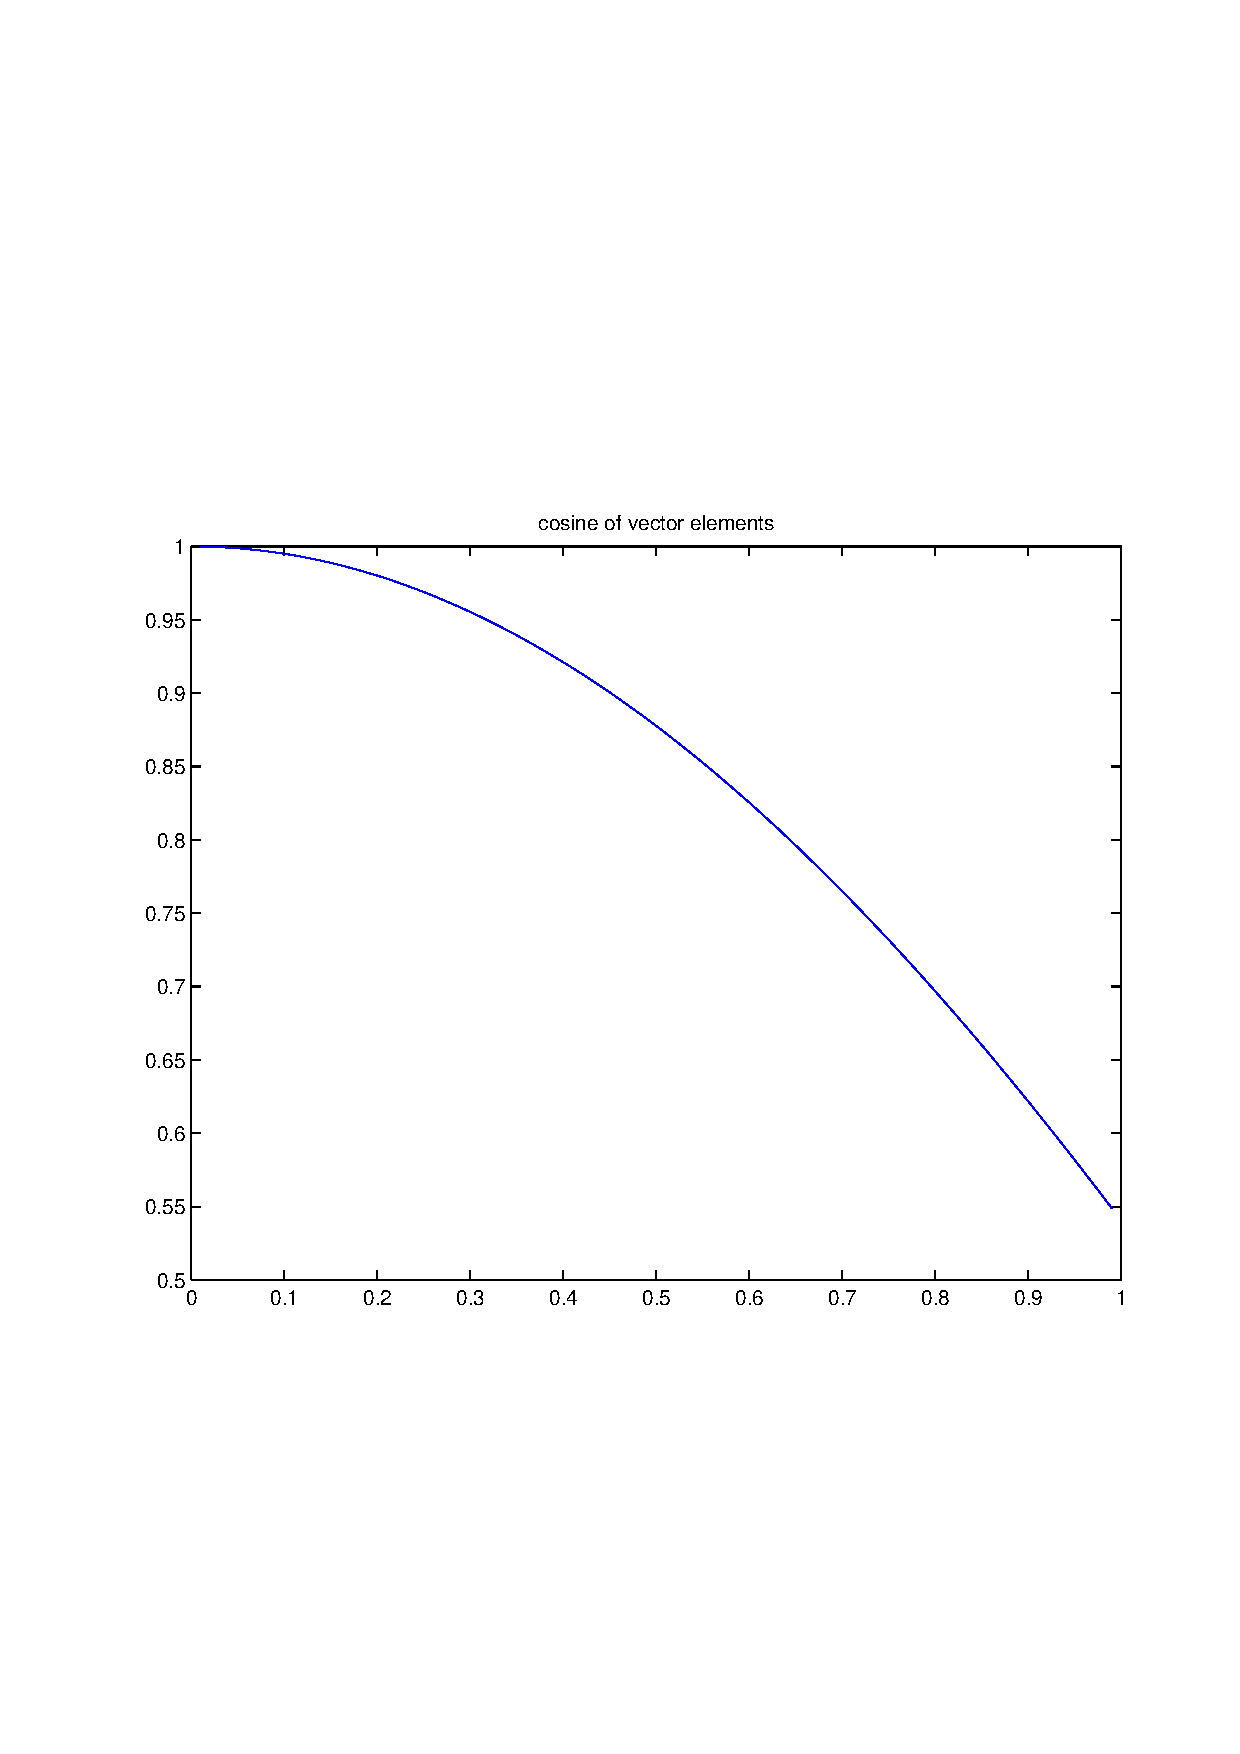
\includegraphics[width=10.0cm,height=10.0cm]{klVSLCos.pdf}

\includegraphics[width=10.0cm,height=10.0cm]{klVSLSin.pdf}

\includegraphics[width=10.0cm,height=10.0cm]{klVSLTan.pdf}

\includegraphics[width=10.0cm,height=10.0cm]{klVSLErf.pdf}

\includegraphics[width=10.0cm,height=10.0cm]{klVSLErfc.pdf}

\includegraphics[width=10.0cm,height=10.0cm]{klVSLCdfNorm.pdf}

\includegraphics[width=10.0cm,height=10.0cm]{klVSLErfInv.pdf}

\includegraphics[width=10.0cm,height=10.0cm]{klVSLLGamma.pdf}

\includegraphics[width=10.0cm,height=10.0cm]{klVSLTGamma.pdf}

QueryPerformanceCounter  =  16.2774
\subsubsection{Gram Matrix Consistency Check}
Sample Size = 4096
Feature dim = 3

$$Sigma$ = \left(
\begin{array}{
ccc}
+1.140 & +1.535 & +0.581 \\
+1.535 & +9.988 & +1.605 \\
+0.581 & +1.605 & +0.428 \\
\end{array}
\right)$ \newline 

$Sample Covariance = \left(
\begin{array}{
ccc}
+1.173 & +1.623 & +0.607 \\
+1.623 & +10.198 & +1.677 \\
+0.607 & +1.677 & +0.449 \\
\end{array}
\right)$ \newline 

$Sample Mean = \left(
\begin{array}{
ccc}
+1.00487 & +1.03891 & +1.00503 \\
\end{array}
\right)$ \newline 

$Sample Covariance-$Omega$ = \left(
\begin{array}{
ccc}
+0.033 & +0.087 & +0.025 \\
+0.087 & +0.209 & +0.072 \\
+0.025 & +0.072 & +0.021 \\
\end{array}
\right)$ \newline 

$Sample Covariance Eigs = \left(
\begin{array}{
ccc}
(+10.77970,+0.00000) & (+0.99995,+0.00000) & (+0.04003,+0.00000) \\
\end{array}
\right)$ \newline 

$Centered Mean = \left(
\begin{array}{
ccc}
+0.00000 & +0.00000 & -0.00000 \\
\end{array}
\right)$ \newline 

$Centered Covariance = \left(
\begin{array}{
ccc}
+1.173 & +1.623 & +0.607 \\
+1.623 & +10.198 & +1.677 \\
+0.607 & +1.677 & +0.449 \\
\end{array}
\right)$ \newline 

$Gram Matrix Gf Not scaled by sample size = \left(
\begin{array}{
ccc}
+4805.998 & +6644.216 & +2485.394 \\
+6644.216 & +41770.290 & +6869.354 \\
+2485.394 & +6869.354 & +1837.099 \\
\end{array}
\right)$ \newline 

$Gram Matrix Gf  scaled by sample size = \left(
\begin{array}{
ccc}
+1.173 & +1.622 & +0.607 \\
+1.622 & +10.198 & +1.677 \\
+0.607 & +1.677 & +0.449 \\
\end{array}
\right)$ \newline 

$SampleCovariance - Scaled Gf = \left(
\begin{array}{
ccc}
+0.000 & +0.000 & +0.000 \\
+0.000 & +0.002 & +0.000 \\
+0.000 & +0.000 & +0.000 \\
\end{array}
\right)$ \newline 

$EigenDecomp of SampleCovariance = \left(
\begin{array}{
ccc}
-0.174 & -0.970 & -0.168 \\
+0.917 & -0.222 & +0.332 \\
-0.360 & -0.096 & +0.928 \\
\end{array}
\right)$ \newline 

$EigenDecomp of Gram Matrix = \left(
\begin{array}{
ccc}
-0.123 & -0.974 & -0.191 \\
-0.328 & +0.222 & -0.918 \\
+0.937 & -0.050 & -0.347 \\
\end{array}
\right)$ \newline 

QueryPerformanceCounter  =  +55.350
\subsubsection{Eigen Solver Checks}
\subsubsection{Haar Distributed Random Orthogonal Matrix $A \in O(n)$}
 Testing Operator Norm
Number of Dimensions: +8

$A = \left(
\begin{array}{
cccccccc}
+0.450 & +0.200 & -0.489 & -0.392 & +0.200 & -0.220 & +0.216 & +0.480 \\
+0.267 & +0.436 & +0.434 & +0.218 & +0.142 & -0.347 & +0.537 & -0.271 \\
+0.447 & -0.285 & +0.297 & -0.415 & +0.473 & +0.072 & -0.321 & -0.356 \\
+0.254 & +0.436 & +0.187 & -0.318 & -0.673 & -0.051 & -0.387 & -0.058 \\
+0.396 & -0.165 & -0.576 & +0.358 & -0.213 & -0.112 & -0.032 & -0.544 \\
-0.116 & -0.567 & +0.140 & -0.236 & -0.296 & -0.692 & +0.148 & +0.034 \\
+0.509 & -0.386 & +0.284 & +0.235 & -0.301 & +0.410 & +0.261 & +0.360 \\
+0.179 & +0.037 & +0.129 & +0.535 & +0.199 & -0.404 & -0.567 & +0.373 \\
\end{array}
\right)$ \newline 

$Det(A) :   A \in O(n)$ = (-1.000,+0.000)

$L = \left(
\begin{array}{
cccccccc}
+1.000 & +0.000 & +0.000 & +0.000 & +0.000 & +0.000 & +0.000 & +0.000 \\
-0.227 & +1.000 & +0.000 & +0.000 & +0.000 & +0.000 & +0.000 & +0.000 \\
+0.777 & -0.205 & +1.000 & +0.000 & +0.000 & +0.000 & +0.000 & +0.000 \\
+0.884 & -0.827 & +0.756 & +1.000 & +0.000 & +0.000 & +0.000 & +0.000 \\
+0.500 & -0.960 & -0.320 & +0.662 & +1.000 & +0.000 & +0.000 & +0.000 \\
+0.524 & -0.975 & -0.642 & -0.007 & +0.086 & +1.000 & +0.000 & +0.000 \\
+0.878 & -0.082 & -0.085 & +0.730 & -0.539 & +0.145 & +1.000 & +0.000 \\
+0.352 & -0.264 & -0.110 & -0.491 & -0.296 & +0.865 & +0.955 & +1.000 \\
\end{array}
\right)$ \newline 

$U = \left(
\begin{array}{
cccccccc}
+0.509 & -0.386 & +0.284 & +0.235 & -0.301 & +0.410 & +0.261 & +0.360 \\
+0.000 & -0.654 & +0.204 & -0.182 & -0.364 & -0.599 & +0.208 & +0.116 \\
+0.000 & +0.000 & -0.755 & +0.138 & -0.054 & -0.553 & -0.192 & -0.800 \\
+0.000 & +0.000 & +0.000 & -0.855 & +0.205 & -0.659 & +0.302 & +0.862 \\
+0.000 & +0.000 & +0.000 & +0.000 & -1.026 & -0.572 & -0.580 & -0.954 \\
+0.000 & +0.000 & +0.000 & +0.000 & +0.000 & -1.457 & +0.532 & -0.772 \\
+0.000 & +0.000 & +0.000 & +0.000 & +0.000 & +0.000 & -1.160 & -1.762 \\
+0.000 & +0.000 & +0.000 & +0.000 & +0.000 & +0.000 & +0.000 & +2.681 \\
\end{array}
\right)$ \newline 

$L * U  = \left(
\begin{array}{
cccccccc}
+0.509 & -0.386 & +0.284 & +0.235 & -0.301 & +0.410 & +0.261 & +0.360 \\
-0.116 & -0.567 & +0.140 & -0.236 & -0.296 & -0.692 & +0.148 & +0.034 \\
+0.396 & -0.165 & -0.576 & +0.358 & -0.213 & -0.112 & -0.032 & -0.544 \\
+0.450 & +0.200 & -0.489 & -0.392 & +0.200 & -0.220 & +0.216 & +0.480 \\
+0.254 & +0.436 & +0.187 & -0.318 & -0.673 & -0.051 & -0.387 & -0.058 \\
+0.267 & +0.436 & +0.434 & +0.218 & +0.142 & -0.347 & +0.537 & -0.271 \\
+0.447 & -0.285 & +0.297 & -0.415 & +0.473 & +0.072 & -0.321 & -0.356 \\
+0.179 & +0.037 & +0.129 & +0.535 & +0.199 & -0.404 & -0.567 & +0.373 \\
\end{array}
\right)$ \newline 

$Det(L) :    = (+1.000,+0.000)     Det(U) :    = (+1.000,+0.000)     Det(LU) :    = (+1.000,+0.000)$

$||A||_{L_1}$  = +2.707

$||A||_{L_{\infty}}$ = +2.745

$||A^{-1}||_{L_1}$  = +2.745

$||A^{-1}||_{L_{\infty}}$ = +2.707

$||A||_{L_{\infty}} * ||A^{-1}||_{L_{\infty}} = +7.431$

$||A||_{L_1} * ||A^{-1}||_{L_1} = +7.431$

Frobenious Norm  $||A||_{\textit{F}}$ via $\sum\limits_{i,j =0}^{n} \|A_{i,j}|$   of  $A \in O(n)$  +2.828

$L_1$ condition number of Haar Distributed Random Orthogonal Matrix $A \in O(n)$ +6.033

$A = \left(
\begin{array}{
cccccccc}
+0.450 & +0.200 & -0.489 & -0.392 & +0.200 & -0.220 & +0.216 & +0.480 \\
+0.267 & +0.436 & +0.434 & +0.218 & +0.142 & -0.347 & +0.537 & -0.271 \\
+0.447 & -0.285 & +0.297 & -0.415 & +0.473 & +0.072 & -0.321 & -0.356 \\
+0.254 & +0.436 & +0.187 & -0.318 & -0.673 & -0.051 & -0.387 & -0.058 \\
+0.396 & -0.165 & -0.576 & +0.358 & -0.213 & -0.112 & -0.032 & -0.544 \\
-0.116 & -0.567 & +0.140 & -0.236 & -0.296 & -0.692 & +0.148 & +0.034 \\
+0.509 & -0.386 & +0.284 & +0.235 & -0.301 & +0.410 & +0.261 & +0.360 \\
+0.179 & +0.037 & +0.129 & +0.535 & +0.199 & -0.404 & -0.567 & +0.373 \\
\end{array}
\right)$ \newline 

$L_{\infty}$ condition number of Haar Distributed Random Orthogonal Matrix $A \in O(n)$ +6.798

Eigenvalues of $A \in O(n)$

(+0.616,+0.788), (+0.616,-0.788), (+0.261,+0.965), (+0.261,-0.965), (-0.580,+0.814), (-0.580,-0.814), (-1.000,+0.000), (+1.000,+0.000)

 $|\lambda | : \lambda \in \sigma(A) , A \in O(n)$

+1.000, +1.000, +1.000, +1.000, +1.000, +1.000, +1.000, +1.000


Calculating $A^{\dag} A,$  we expect $A^{\dag} A \approx I$

$A^{\dag} A = \left(
\begin{array}{
cccccccc}
+1.000 & +0.000 & -0.000 & -0.000 & +0.000 & -0.000 & +0.000 & +0.000 \\
+0.000 & +1.000 & -0.000 & -0.000 & -0.000 & -0.000 & -0.000 & +0.000 \\
-0.000 & -0.000 & +1.000 & +0.000 & -0.000 & +0.000 & +0.000 & -0.000 \\
-0.000 & -0.000 & +0.000 & +1.000 & +0.000 & -0.000 & -0.000 & -0.000 \\
+0.000 & -0.000 & -0.000 & +0.000 & +1.000 & -0.000 & +0.000 & -0.000 \\
-0.000 & -0.000 & +0.000 & -0.000 & -0.000 & +1.000 & +0.000 & -0.000 \\
+0.000 & -0.000 & +0.000 & -0.000 & +0.000 & +0.000 & +1.000 & +0.000 \\
+0.000 & +0.000 & -0.000 & -0.000 & -0.000 & -0.000 & +0.000 & +1.000 \\
\end{array}
\right)$ \newline 

Calculating $A^{-1} ,  A \in O(n)$.

$A^{-1} = \left(
\begin{array}{
cccccccc}
+0.450 & +0.267 & +0.447 & +0.254 & +0.396 & -0.116 & +0.509 & +0.179 \\
+0.200 & +0.436 & -0.285 & +0.436 & -0.165 & -0.567 & -0.386 & +0.037 \\
-0.489 & +0.434 & +0.297 & +0.187 & -0.576 & +0.140 & +0.284 & +0.129 \\
-0.392 & +0.218 & -0.415 & -0.318 & +0.358 & -0.236 & +0.235 & +0.535 \\
+0.200 & +0.142 & +0.473 & -0.673 & -0.213 & -0.296 & -0.301 & +0.199 \\
-0.220 & -0.347 & +0.072 & -0.051 & -0.112 & -0.692 & +0.410 & -0.404 \\
+0.216 & +0.537 & -0.321 & -0.387 & -0.032 & +0.148 & +0.261 & -0.567 \\
+0.480 & -0.271 & -0.356 & -0.058 & -0.544 & +0.034 & +0.360 & +0.373 \\
\end{array}
\right)$ \newline 

Calculating $A^{-1} *A  ,  A \in O(n)$.   We expect $A^{-1} *A  \approx I$. 

$A^{-1} *A = \left(
\begin{array}{
cccccccc}
+1.000 & +0.000 & -0.000 & -0.000 & +0.000 & -0.000 & +0.000 & -0.000 \\
+0.000 & +1.000 & +0.000 & +0.000 & +0.000 & -0.000 & +0.000 & -0.000 \\
+0.000 & +0.000 & +1.000 & -0.000 & +0.000 & -0.000 & +0.000 & -0.000 \\
+0.000 & -0.000 & -0.000 & +1.000 & -0.000 & -0.000 & -0.000 & -0.000 \\
+0.000 & -0.000 & -0.000 & -0.000 & +1.000 & +0.000 & -0.000 & -0.000 \\
+0.000 & -0.000 & +0.000 & -0.000 & +0.000 & +1.000 & -0.000 & +0.000 \\
+0.000 & +0.000 & -0.000 & +0.000 & -0.000 & +0.000 & +1.000 & +0.000 \\
-0.000 & +0.000 & +0.000 & +0.000 & -0.000 & +0.000 & -0.000 & +1.000 \\
\end{array}
\right)$ \newline 

Calculating SVD of  $A \in O(n)$

$U = \left(
\begin{array}{
cccccccc}
-0.450 & -0.200 & +0.489 & +0.392 & -0.200 & +0.220 & -0.216 & -0.480 \\
-0.261 & -0.446 & +0.242 & +0.048 & +0.043 & -0.538 & -0.249 & +0.564 \\
-0.292 & +0.545 & +0.238 & +0.272 & -0.082 & +0.304 & +0.243 & +0.574 \\
-0.265 & +0.509 & +0.024 & -0.404 & -0.481 & -0.446 & -0.211 & -0.178 \\
+0.631 & +0.040 & +0.692 & -0.230 & -0.145 & +0.112 & -0.161 & +0.093 \\
+0.115 & -0.369 & -0.213 & +0.066 & -0.825 & +0.132 & +0.279 & +0.160 \\
-0.386 & -0.241 & +0.033 & -0.720 & +0.076 & +0.499 & -0.048 & +0.126 \\
+0.117 & +0.099 & -0.346 & +0.176 & -0.116 & +0.303 & -0.825 & +0.199 \\
\end{array}
\right)$ \newline 

$S = \left(
\begin{array}{
cccccccc}
+1.000 & +0.000 & +0.000 & +0.000 & +0.000 & +0.000 & +0.000 & +0.000 \\
+0.000 & +1.000 & +0.000 & +0.000 & +0.000 & +0.000 & +0.000 & +0.000 \\
+0.000 & +0.000 & +1.000 & +0.000 & +0.000 & +0.000 & +0.000 & +0.000 \\
+0.000 & +0.000 & +0.000 & +1.000 & +0.000 & +0.000 & +0.000 & +0.000 \\
+0.000 & +0.000 & +0.000 & +0.000 & +1.000 & +0.000 & +0.000 & +0.000 \\
+0.000 & +0.000 & +0.000 & +0.000 & +0.000 & +1.000 & +0.000 & +0.000 \\
+0.000 & +0.000 & +0.000 & +0.000 & +0.000 & +0.000 & +1.000 & +0.000 \\
+0.000 & +0.000 & +0.000 & +0.000 & +0.000 & +0.000 & +0.000 & +1.000 \\
\end{array}
\right)$ \newline 

$V = \left(
\begin{array}{
cccccccc}
-1.000 & -0.000 & +0.000 & -0.000 & -0.000 & +0.000 & -0.000 & -0.000 \\
-0.000 & -0.243 & +0.180 & +0.095 & +0.265 & -0.265 & -0.573 & -0.656 \\
-0.000 & -0.076 & -0.627 & -0.217 & +0.530 & -0.461 & +0.247 & +0.009 \\
+0.000 & -0.169 & +0.033 & +0.726 & +0.530 & +0.239 & -0.033 & +0.323 \\
+0.000 & -0.400 & -0.582 & -0.092 & -0.265 & +0.318 & -0.529 & +0.202 \\
+0.000 & +0.648 & -0.437 & +0.255 & +0.000 & +0.350 & -0.015 & -0.450 \\
+0.000 & +0.023 & +0.192 & -0.577 & +0.530 & +0.589 & -0.049 & -0.020 \\
+0.000 & +0.572 & +0.081 & -0.104 & +0.132 & -0.301 & -0.572 & +0.470 \\
\end{array}
\right)$ \newline 

$U S V = \left(
\begin{array}{
cccccccc}
+0.450 & -0.112 & -0.390 & +0.409 & +0.288 & -0.048 & +0.609 & -0.098 \\
+0.261 & +0.032 & -0.023 & -0.116 & -0.034 & -0.473 & -0.011 & +0.832 \\
+0.292 & +0.368 & -0.034 & +0.082 & +0.641 & -0.139 & -0.564 & -0.156 \\
+0.265 & -0.260 & +0.483 & -0.180 & -0.075 & -0.622 & +0.101 & -0.440 \\
-0.631 & +0.156 & -0.422 & -0.188 & +0.221 & -0.514 & +0.186 & -0.127 \\
-0.115 & +0.608 & +0.559 & -0.009 & +0.212 & +0.112 & +0.486 & +0.105 \\
+0.386 & +0.541 & -0.349 & -0.418 & -0.457 & +0.009 & +0.053 & -0.223 \\
-0.117 & +0.310 & +0.034 & +0.755 & -0.444 & -0.301 & -0.164 & -0.061 \\
\end{array}
\right)$ \newline 

Calculating first few eigenvectors of $A \in O(n)$ using LAPACK syevx

\subsubsection{Wishart Matrix $A \in W(n)$}
$L_1$ condition number of Wishart Matrix +1489.694
$L_infty$ condition number of Wishart Matrix +1489.694
\subsubsection{Gaussian Orthogonal Ensemble $A \in GOE(n)$}
$L_1$ condition number of GOE Matrix +66.900
$L_\infty$ condition number of GOE Matrix +66.900
\subsubsection{The Identity Matrix $I \in M(n)$}
$L_1$ condition number of $I$ = +1.000
$L_\infty$ condition number of $I$ = +1.000
QueryPerformanceCounter  =  +1.910
\subsubsection{Generate Tracey Widom Sample}
\subsubsection{Sample from $W_n m$ times and calculate empirical PDF of the first eig}
Here we generate histograms of $\lambda_1$ for GOE (Gaussian Orthogonal Ensemble), and W (Wishart) 		 distributed of random matrices
These should approximate the celebrated Tracy Widom distribution.
Dimension $n = +128$

Sample size $m = 32$

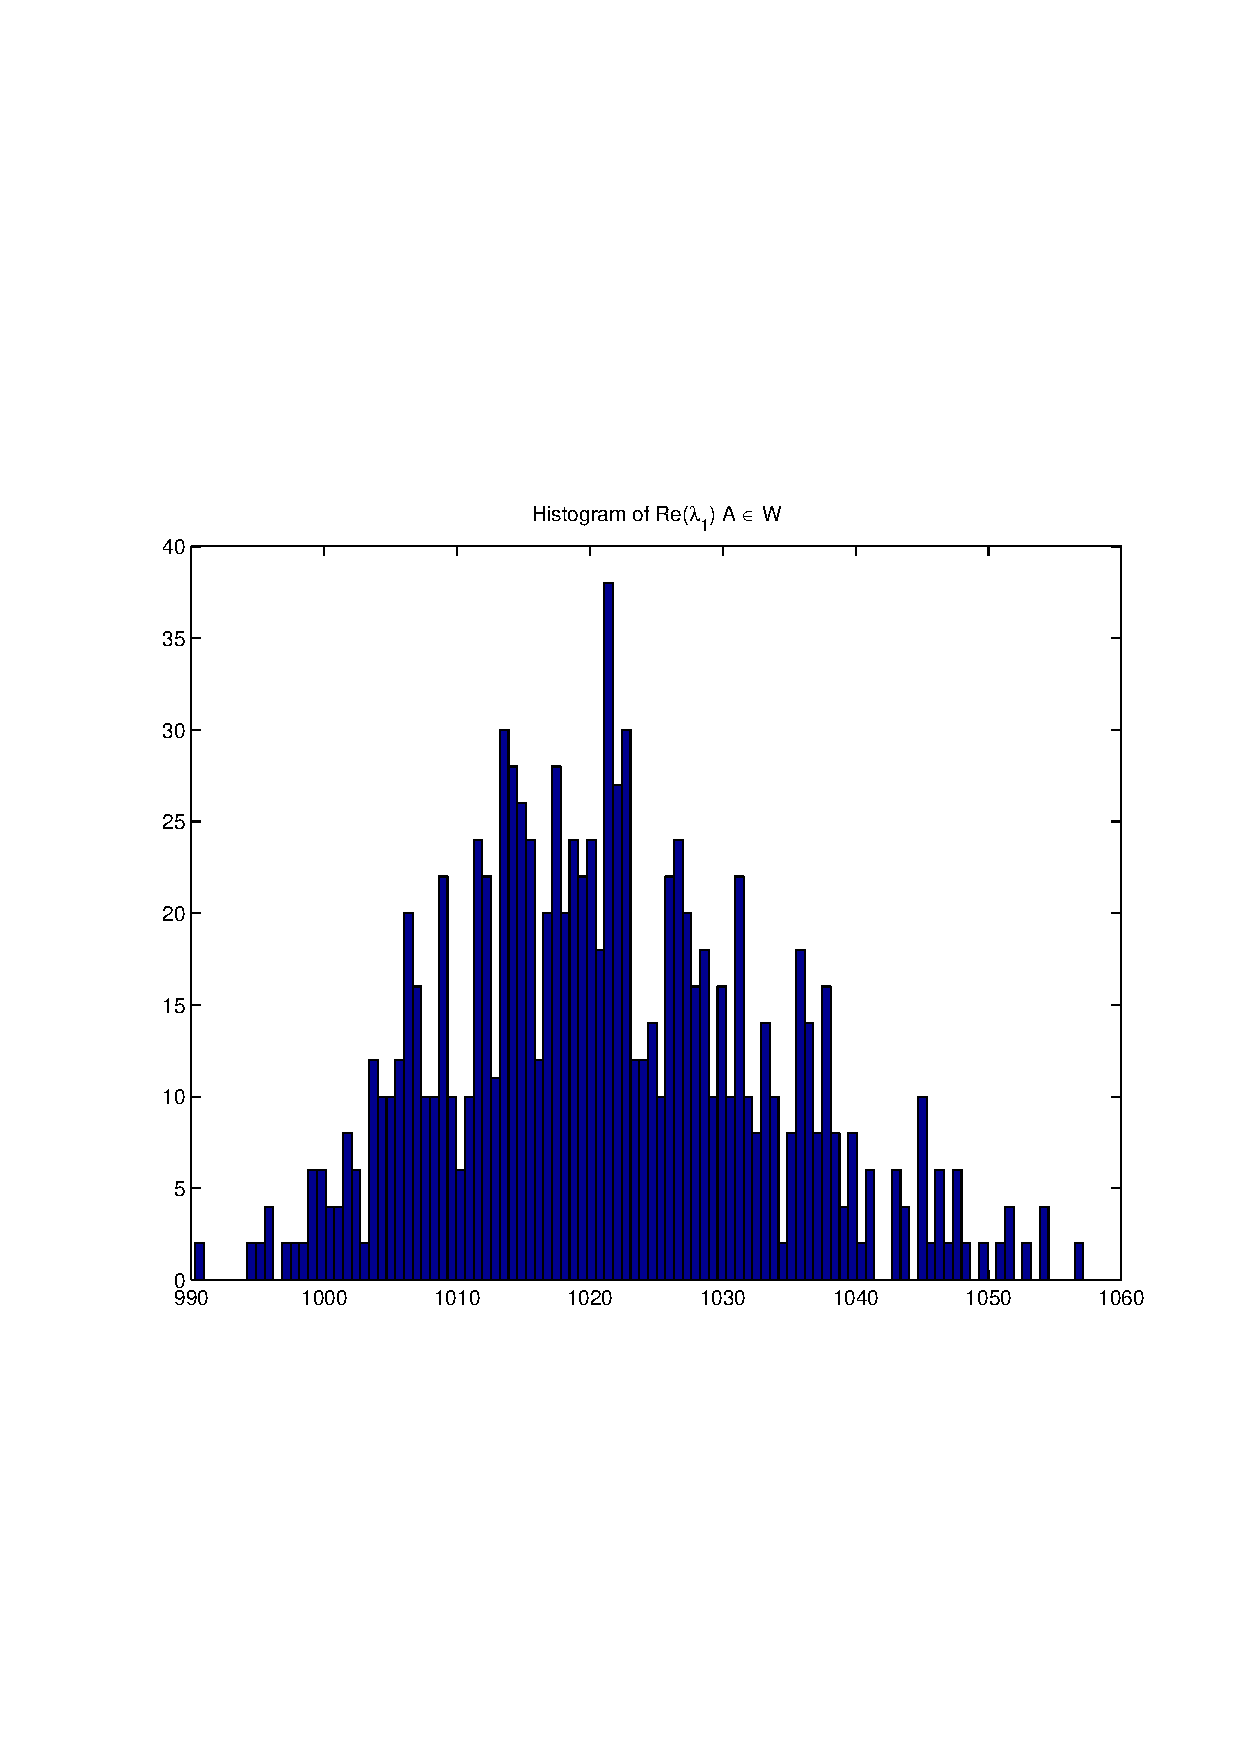
\includegraphics[width=10.0cm,height=10.0cm]{Re_TraceyWidom.pdf}

\includegraphics[width=10.0cm,height=10.0cm]{Im_TraceyWidom.pdf}

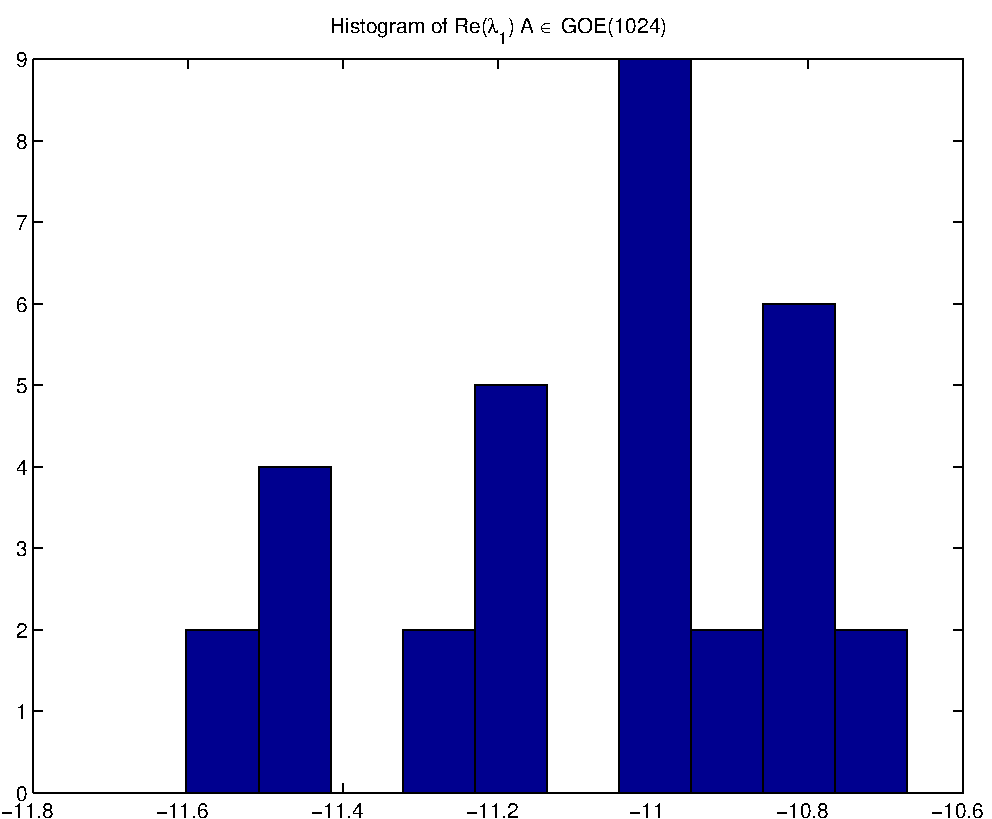
\includegraphics[width=10.0cm,height=10.0cm]{Re_Winger.pdf}

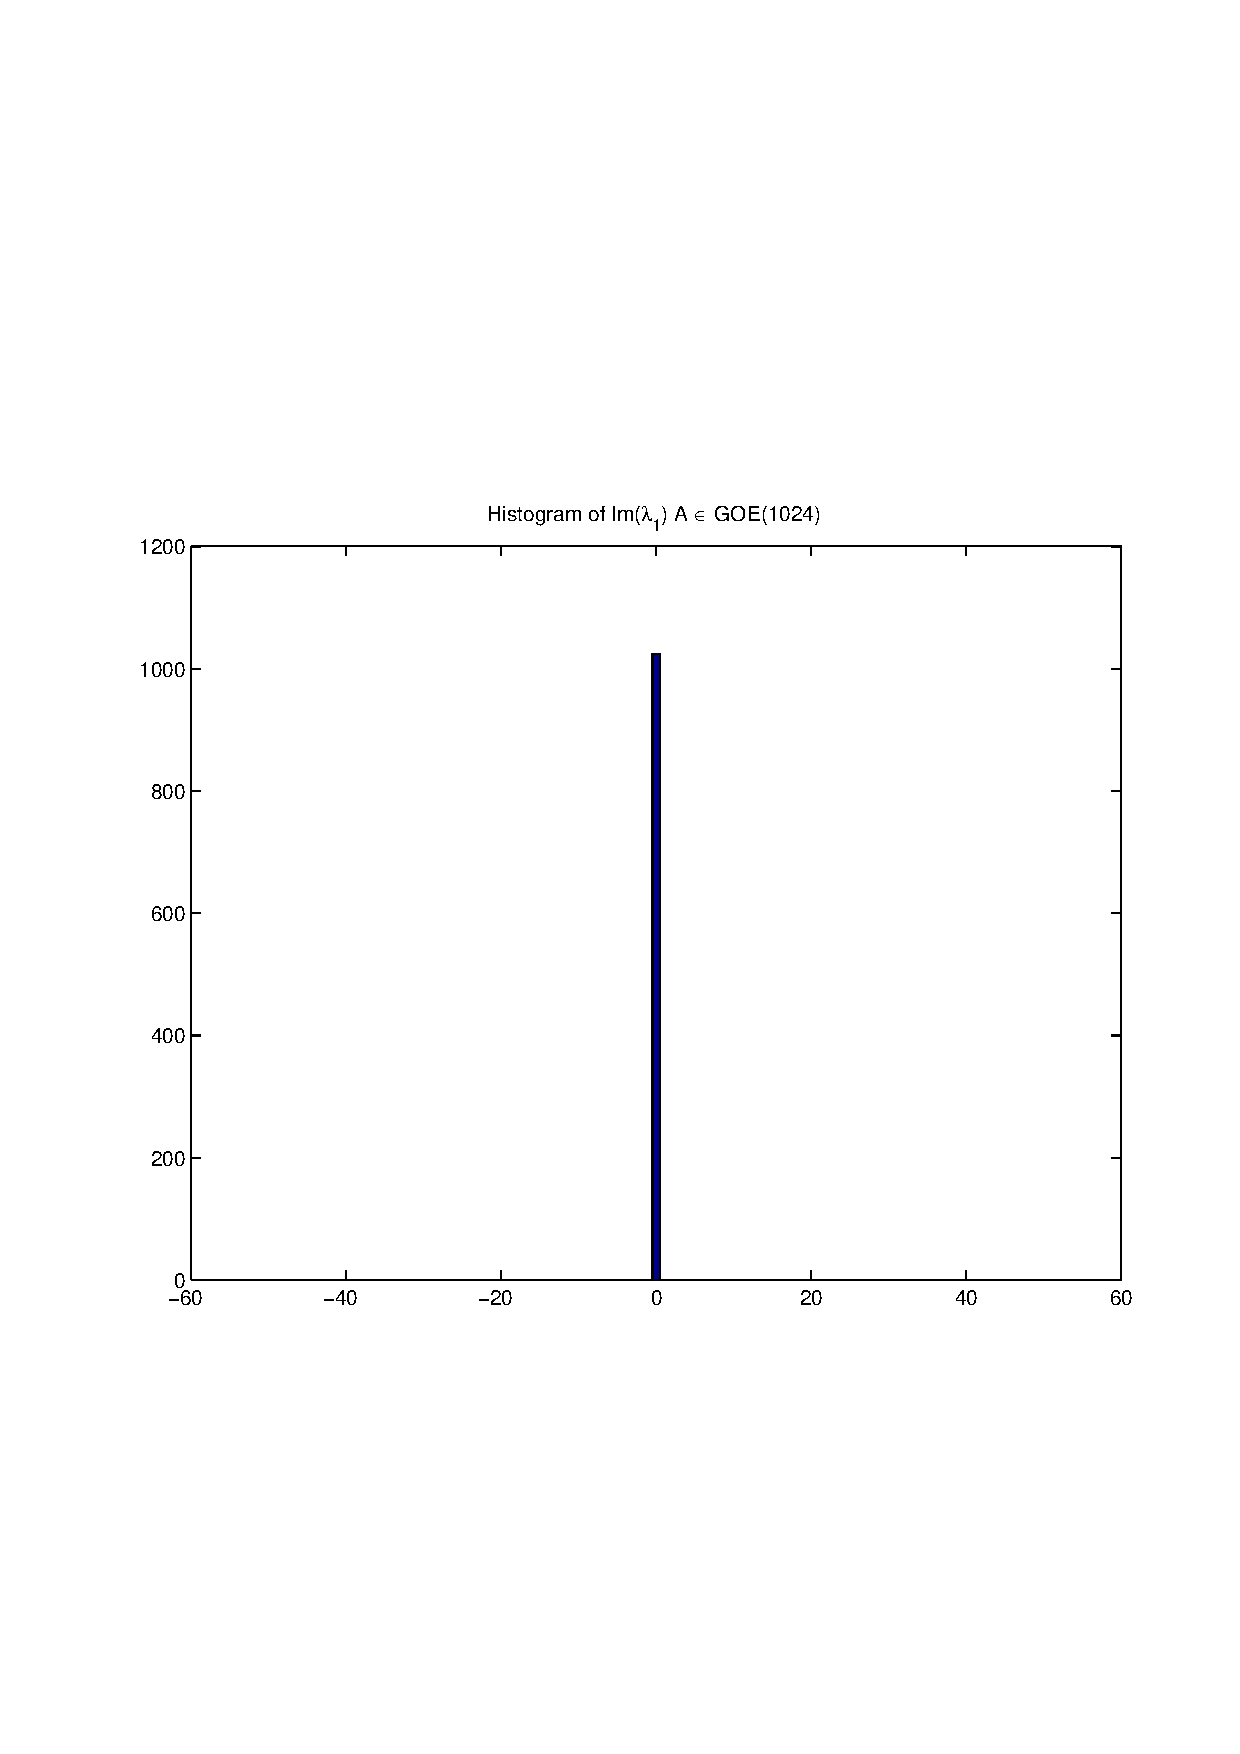
\includegraphics[width=10.0cm,height=10.0cm]{Im_Winger.pdf}

QueryPerformanceCounter  =  +10.085
\subsubsection{Approximate Winger Distribution}
\subsubsection{Verfy Winger Law.}
Let $M_n = [X_{ij} ]$ a symmetric n x n matrix with Random entries such that $X_{i,j} = X_{j,i}$, 		  and $X_{i,j}$ are iid $orall i < j,$ and $Xjj$ are iid $orall j  :  ; E[X^2_{ij} ] = 1, & E[X_{ij}] = 0$ 		  and that all moments exists for each of the entries.  		  The eigenvector of this random matrix; $ lambda_1 leq ... leq lambda_n$ depends continuously on $Mn$.
Dimension $n = +512$

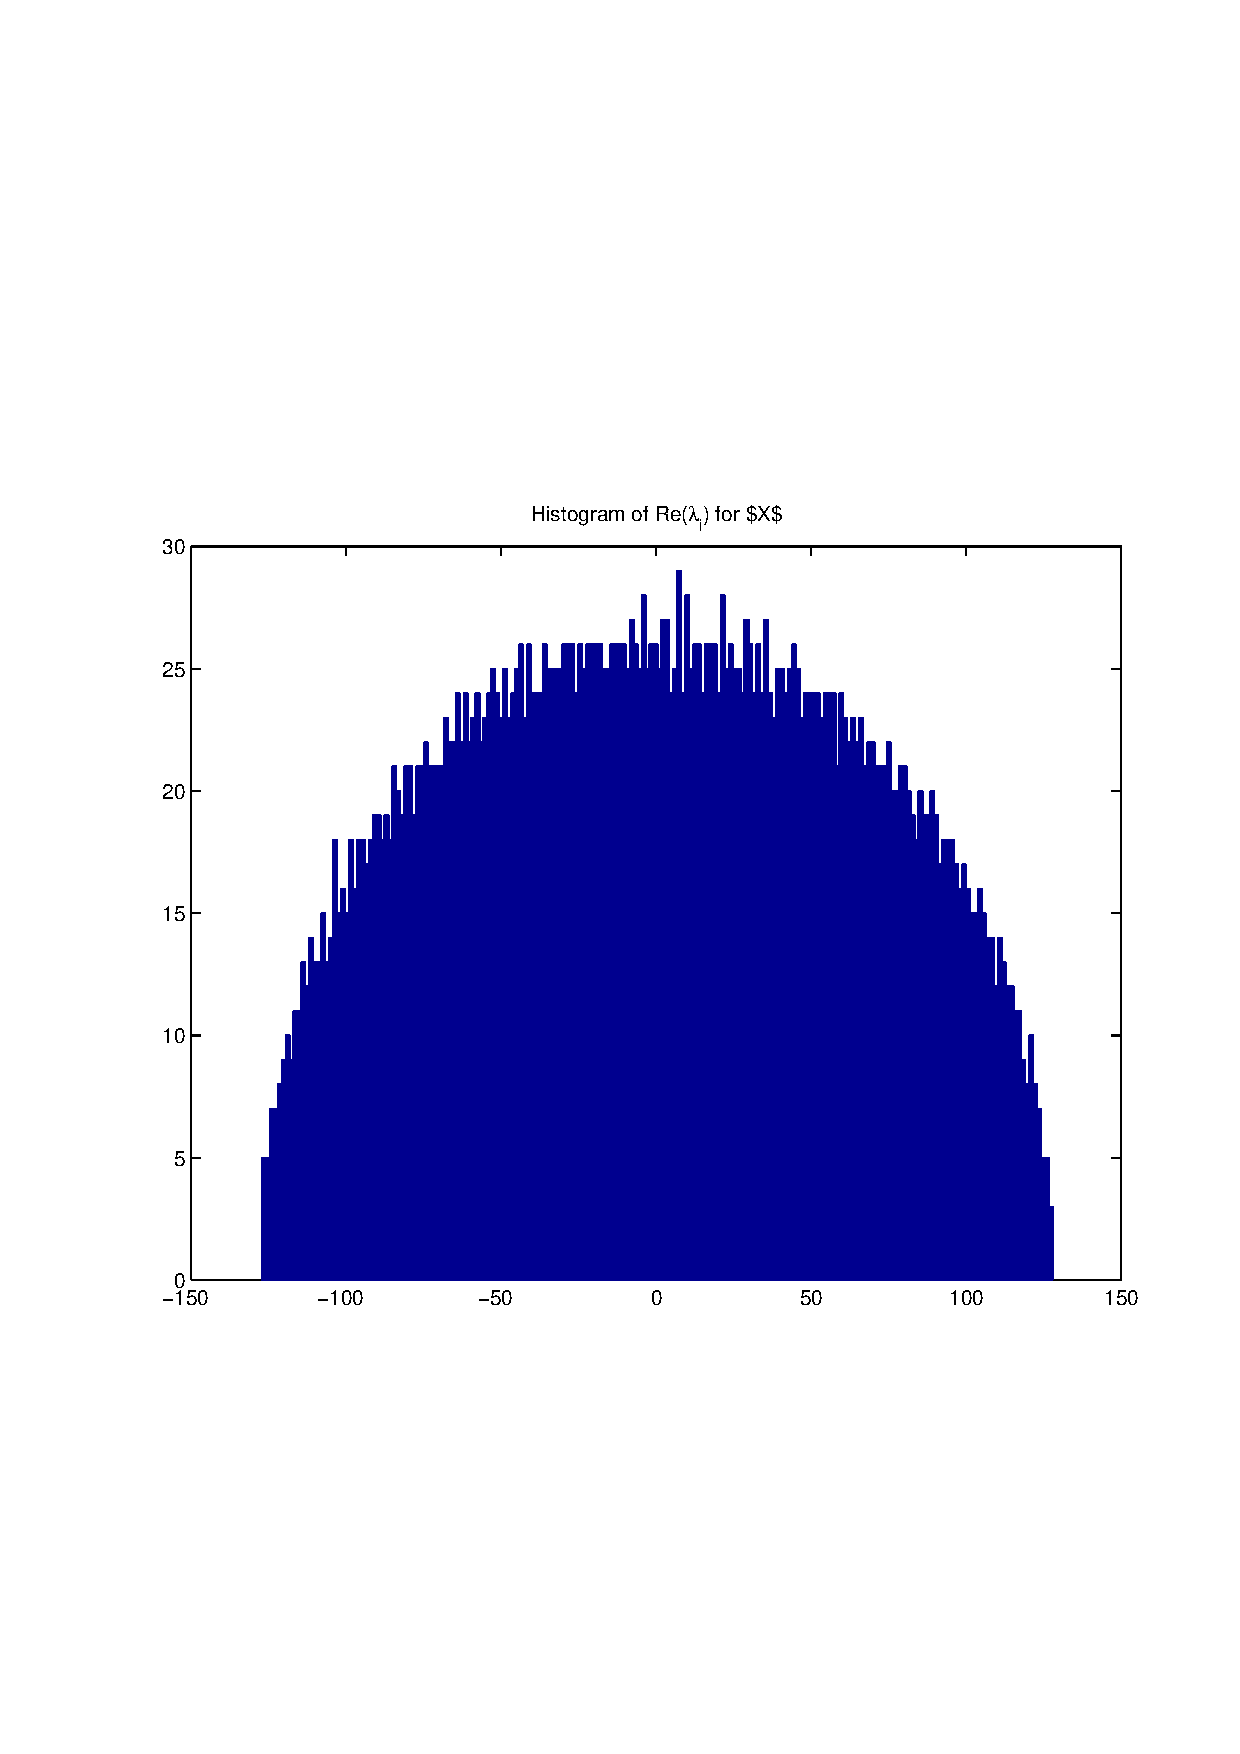
\includegraphics[width=10.0cm,height=10.0cm]{Re_lambda_n.pdf}

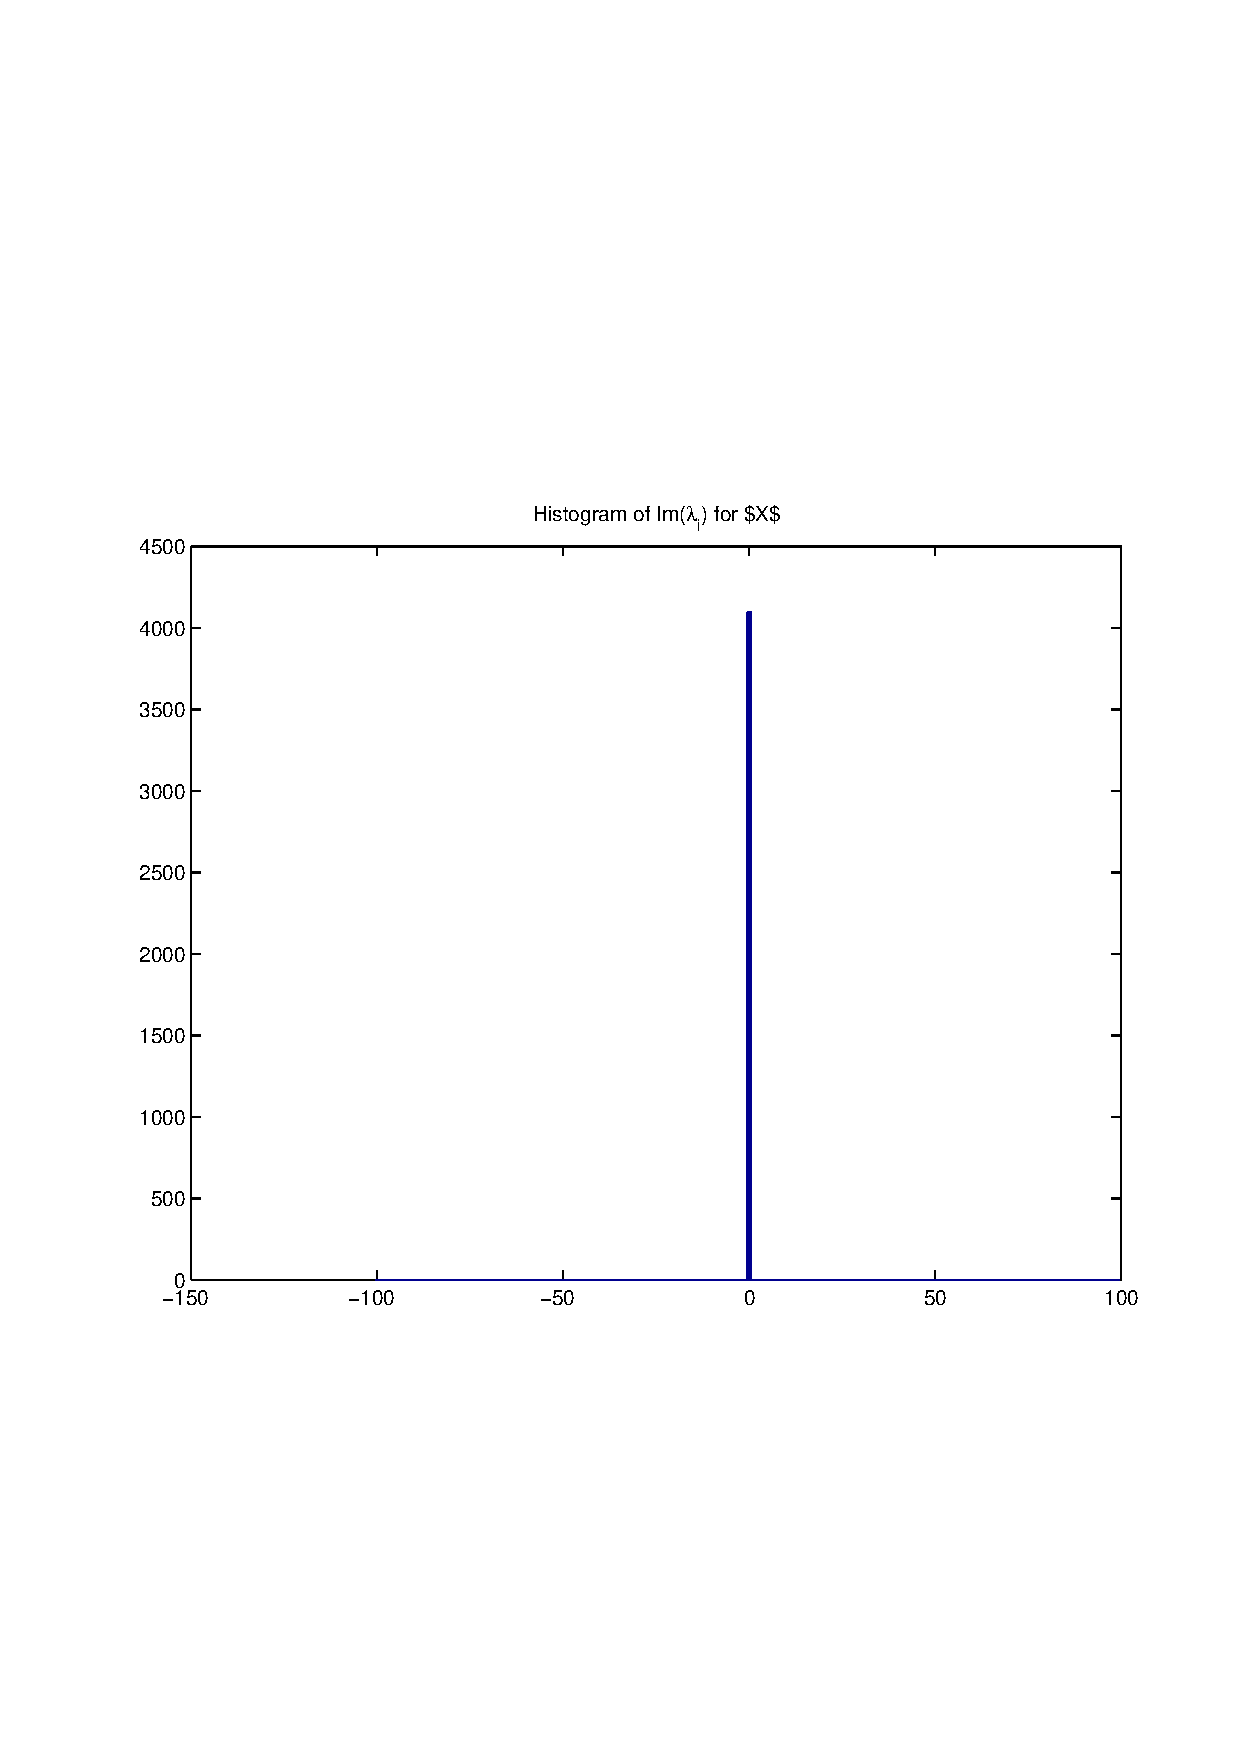
\includegraphics[width=10.0cm,height=10.0cm]{Im_lambda_n.pdf}

QueryPerformanceCounter  =  +3.071
\subsubsection{Iterated Exponential Filtering }
$\mu_1 =+0.093$
$\mu_2 =+0.726$
$\mu_3 =+0.011$
$\mu_4 =+2.178$
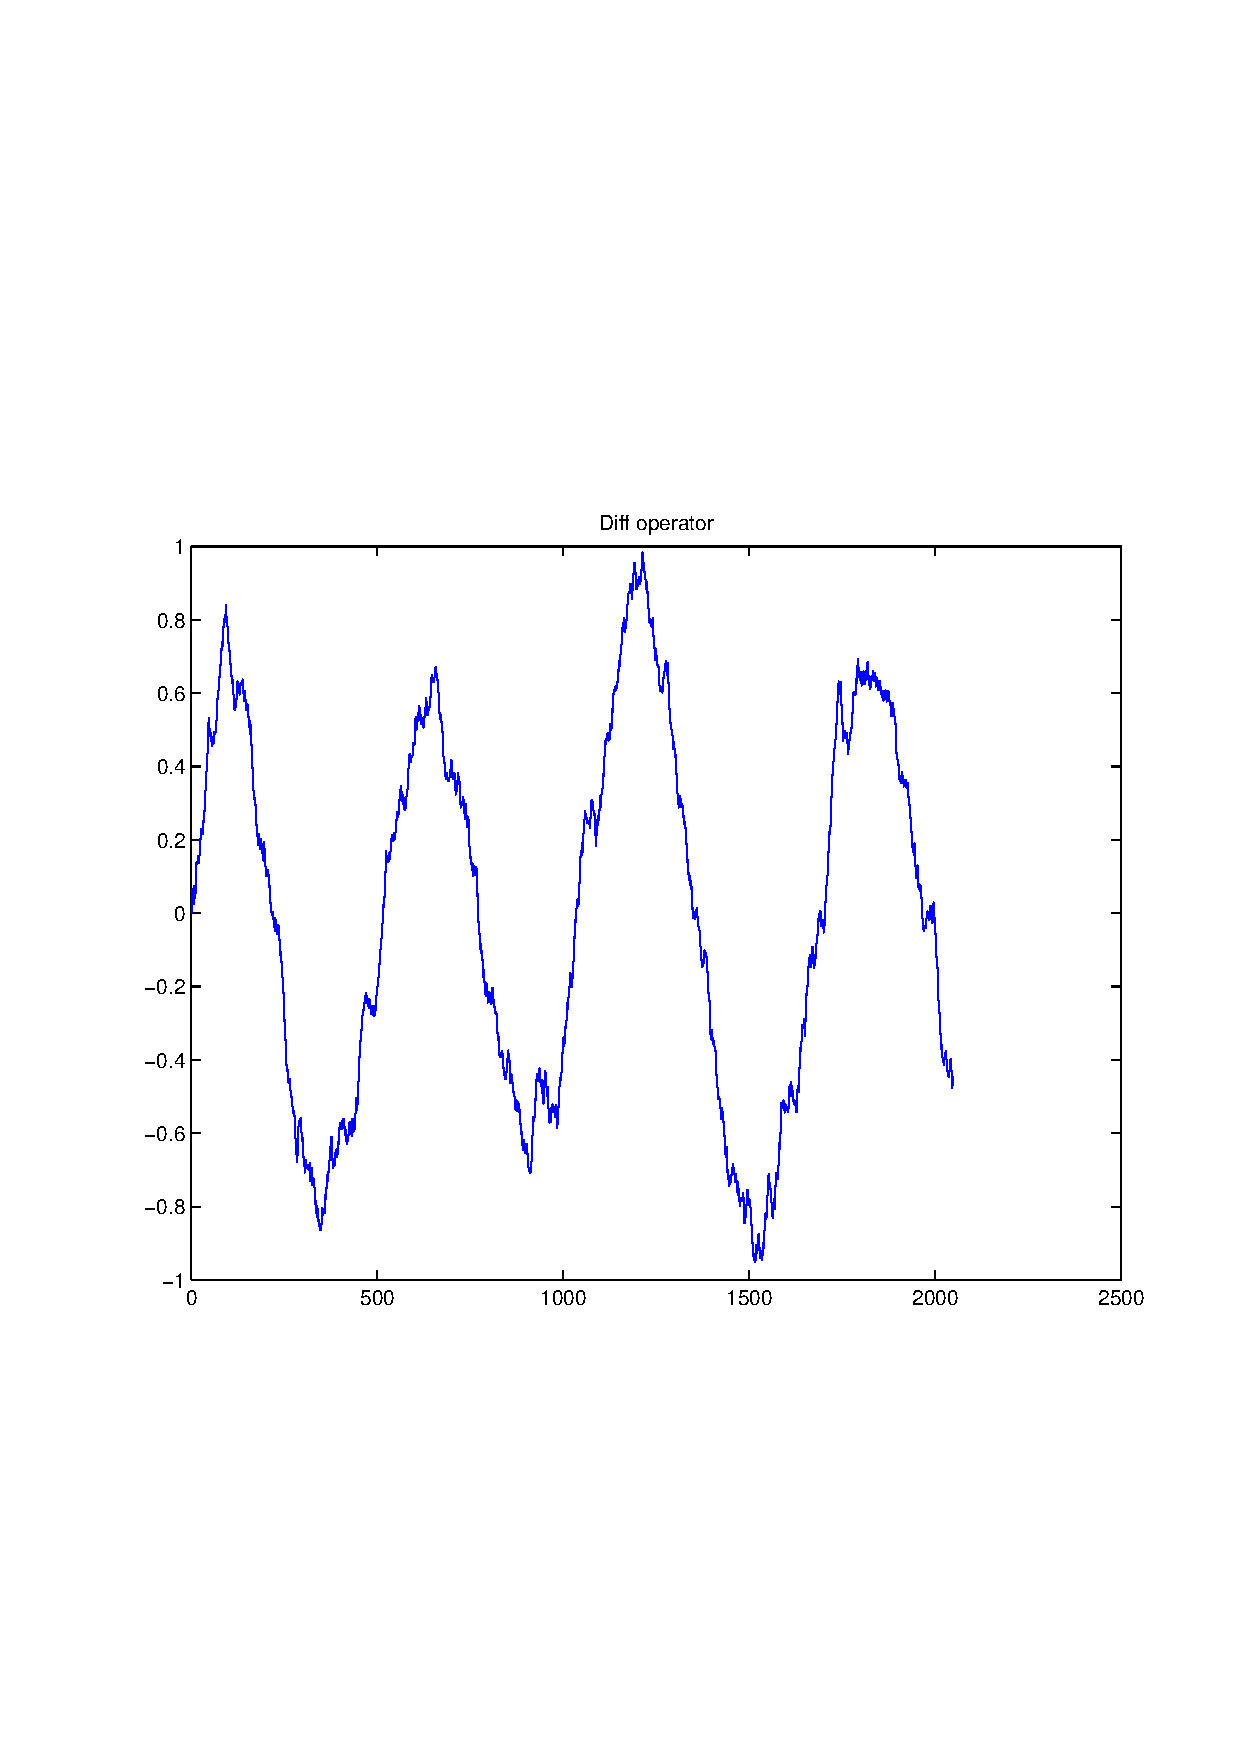
\includegraphics[width=10.0cm,height=10.0cm]{DIFF.pdf}

QueryPerformanceCounter  =  +1.678
\subsubsection{Matrix Exponential }
$SPD Matrix = \left(
\begin{array}{
cccccccc}
+10.539 & -0.499 & -0.010 & +0.368 & +0.465 & -0.492 & -0.126 & +0.437 \\
-0.499 & +7.286 & +0.365 & -0.481 & -0.337 & -0.466 & +0.279 & +0.056 \\
-0.010 & +0.365 & +6.705 & -0.205 & +0.467 & +0.131 & +0.077 & -0.089 \\
+0.368 & -0.481 & -0.205 & +6.496 & -0.402 & -0.209 & +0.043 & -0.041 \\
+0.465 & -0.337 & +0.467 & -0.402 & +4.578 & +0.272 & +0.289 & -0.285 \\
-0.492 & -0.466 & +0.131 & -0.209 & +0.272 & +8.181 & +0.343 & -0.244 \\
-0.126 & +0.279 & +0.077 & +0.043 & +0.289 & +0.343 & +5.938 & -0.212 \\
+0.437 & +0.056 & -0.089 & -0.041 & -0.285 & -0.244 & -0.212 & +9.691 \\
\end{array}
\right)$ \newline 

$SPD Eigs = \left(
\begin{array}{
cccccccc}
(+10.93611,+0.00000) & (+9.60778,+0.00000) & (+4.23666,+0.00000) & (+8.36911,+0.00000) & (+7.56229,+0.00000) & (+5.82791,+0.00000) & (+6.54198,+0.00000) & (+6.33139,+0.00000) \\
\end{array}
\right)$ \newline 

$exp(SPD) = \left(
\begin{array}{
cccccccc}
+47863.969 & -6460.093 & -1078.770 & +4706.958 & +2535.224 & -8475.398 & -2406.368 & +12977.552 \\
-6460.093 & +2780.574 & +516.920 & -1069.918 & -548.083 & -109.707 & +386.466 & -807.216 \\
-1078.770 & +516.920 & +1015.281 & -385.755 & +176.069 & +458.541 & +212.284 & -859.022 \\
+4706.958 & -1069.918 & -385.755 & +1267.210 & +111.181 & -1018.272 & -287.809 & +1036.628 \\
+2535.224 & -548.083 & +176.069 & +111.181 & +413.265 & +135.193 & +45.490 & -502.411 \\
-8475.398 & -109.707 & +458.541 & -1018.272 & +135.193 & +5613.026 & +968.003 & -4270.737 \\
-2406.368 & +386.466 & +212.284 & -287.809 & +45.490 & +968.003 & +632.432 & -1645.725 \\
+12977.552 & -807.216 & -859.022 & +1036.628 & -502.411 & -4270.737 & -1645.725 & +19362.944 \\
\end{array}
\right)$ \newline 

$exp(SPD) eigs = \left(
\begin{array}{
cccccccc}
(+56168.17045,+0.00000) & (+14880.07985,+0.00000) & (+4311.77579,+0.00000) & (+1924.25027,+0.00000) & (+69.17669,+0.00000) & (+339.64809,+0.00000) & (+693.66208,+0.00000) & (+561.93669,+0.00000) \\
\end{array}
\right)$ \newline 

$log(exp(SPD) eigs)  = \left(
\begin{array}{
cccccccc}
(+10.93611,+0.00000) & (+9.60778,+0.00000) & (+8.36911,+0.00000) & (+7.56229,+0.00000) & (+4.23666,+0.00000) & (+5.82791,+0.00000) & (+6.54198,+0.00000) & (+6.33139,+0.00000) \\
\end{array}
\right)$ \newline 

$exp(Id) = \left(
\begin{array}{
cccccccc}
+2.718 & +0.000 & +0.000 & +0.000 & +0.000 & +0.000 & +0.000 & +0.000 \\
+0.000 & +2.718 & +0.000 & +0.000 & +0.000 & +0.000 & +0.000 & +0.000 \\
+0.000 & +0.000 & +2.718 & +0.000 & +0.000 & +0.000 & +0.000 & +0.000 \\
+0.000 & +0.000 & +0.000 & +2.718 & +0.000 & +0.000 & +0.000 & +0.000 \\
+0.000 & +0.000 & +0.000 & +0.000 & +2.718 & +0.000 & +0.000 & +0.000 \\
+0.000 & +0.000 & +0.000 & +0.000 & +0.000 & +2.718 & +0.000 & +0.000 \\
+0.000 & +0.000 & +0.000 & +0.000 & +0.000 & +0.000 & +2.718 & +0.000 \\
+0.000 & +0.000 & +0.000 & +0.000 & +0.000 & +0.000 & +0.000 & +2.718 \\
\end{array}
\right)$ \newline 

$exp(Id) eigs = \left(
\begin{array}{
cccccccc}
(+2.71828,+0.00000) & (+2.71828,+0.00000) & (+2.71828,+0.00000) & (+2.71828,+0.00000) & (+2.71828,+0.00000) & (+2.71828,+0.00000) & (+2.71828,+0.00000) & (+2.71828,+0.00000) \\
\end{array}
\right)$ \newline 

$log(exp(Id) eigs)  = \left(
\begin{array}{
cccccccc}
(+1.00000,+0.00000) & (+1.00000,+0.00000) & (+1.00000,+0.00000) & (+1.00000,+0.00000) & (+1.00000,+0.00000) & (+1.00000,+0.00000) & (+1.00000,+0.00000) & (+1.00000,+0.00000) \\
\end{array}
\right)$ \newline 

For $n  \in  \dblz [16,128)$ we calculate  $|( SPD(n) Eigs - log(exp(SPD(n)) eigs)|_{l^2}$

$|( SPD(n) Eigs - log(exp(SPD(n)) eigs)|_{l^2} = \left(
\begin{array}{
cccccccccccccccccccccccccccccccccccccccccccccccccccccccccccccccccccccccccccccccccccccccccccccccccccccccccccccccc}
(+5.36543,+0.00000) & (+5.36543,+0.00000) & (+5.36543,+0.00000) & (+5.36543,+0.00000) & (+5.36543,+0.00000) & (+5.36543,+0.00000) & (+5.36543,+0.00000) & (+5.36543,+0.00000) & (+5.36543,+0.00000) & (+5.36543,+0.00000) & (+5.36543,+0.00000) & (+5.36543,+0.00000) & (+5.36543,+0.00000) & (+5.36543,+0.00000) & (+5.36543,+0.00000) & (+5.36543,+0.00000) & (+5.36543,+0.00000) & (+5.36543,+0.00000) & (+5.36543,+0.00000) & (+5.36543,+0.00000) & (+5.36543,+0.00000) & (+5.36543,+0.00000) & (+5.36543,+0.00000) & (+5.36543,+0.00000) & (+5.36543,+0.00000) & (+5.36543,+0.00000) & (+5.36543,+0.00000) & (+5.36543,+0.00000) & (+5.36543,+0.00000) & (+5.36543,+0.00000) & (+5.36543,+0.00000) & (+5.36543,+0.00000) & (+5.36543,+0.00000) & (+5.36543,+0.00000) & (+5.36543,+0.00000) & (+5.36543,+0.00000) & (+5.36543,+0.00000) & (+5.36543,+0.00000) & (+5.36543,+0.00000) & (+5.36543,+0.00000) & (+5.36543,+0.00000) & (+5.36543,+0.00000) & (+5.36543,+0.00000) & (+5.36543,+0.00000) & (+5.36543,+0.00000) & (+5.36543,+0.00000) & (+5.36543,+0.00000) & (+5.36543,+0.00000) & (+0.00000,+0.00000) & (+0.00000,+0.00000) & (+0.00000,+0.00000) & (+0.00000,+0.00000) & (+0.00000,+0.00000) & (+0.00000,+0.00000) & (+0.00000,+0.00000) & (+0.00000,+0.00000) & (+0.00000,+0.00000) & (+0.00000,+0.00000) & (+0.00000,+0.00000) & (+0.00000,+0.00000) & (+0.00000,+0.00000) & (+0.00000,+0.00000) & (+0.00000,+0.00000) & (+0.00000,+0.00000) & (+0.00000,+0.00000) & (+0.00000,+0.00000) & (+0.00000,+0.00000) & (+0.00000,+0.00000) & (+0.00000,+0.00000) & (+0.00000,+0.00000) & (+0.00000,+0.00000) & (+0.00000,+0.00000) & (+0.00000,+0.00000) & (+0.00000,+0.00000) & (+0.00000,+0.00000) & (+0.00000,+0.00000) & (+0.00000,+0.00000) & (+0.00000,+0.00000) & (+0.00000,+0.00000) & (+0.00000,+0.00000) & (+0.00000,+0.00000) & (+0.00000,+0.00000) & (+0.00000,+0.00000) & (+0.00000,+0.00000) & (+0.00000,+0.00000) & (+0.00000,+0.00000) & (+0.00000,+0.00000) & (+0.00000,+0.00000) & (+0.00000,+0.00000) & (+0.00000,+0.00000) & (+0.00000,+0.00000) & (+0.00000,+0.00000) & (+0.00000,+0.00000) & (+0.00000,+0.00000) & (+0.00000,+0.00000) & (+0.00000,+0.00000) & (+0.00000,+0.00000) & (+0.00000,+0.00000) & (+0.00000,+0.00000) & (+0.00000,+0.00000) & (+0.00000,+0.00000) & (+0.00000,+0.00000) & (+0.00000,+0.00000) & (+0.00000,+0.00000) & (+0.00000,+0.00000) & (+0.00000,+0.00000) & (+0.00000,+0.00000) & (+0.00000,+0.00000) & (+0.00000,+0.00000) & (+0.00000,+0.00000) & (+0.00000,+0.00000) & (+0.00000,+0.00000) \\
\end{array}
\right)$ \newline 

QueryPerformanceCounter  =  +0.04728
The sample size generated for this run is 100000.

\newpage
uniform \begin{tabular}{|c|c|c|c|}  mean & variance & skewness & kurtosis \\  \hline
$\mu_1 = +0.50030$ & $\mu_2 = +0.08353$ & $\mu_3 = +0.00339$ & $\mu_4 =+1.80113$ \\
\end{tabular}

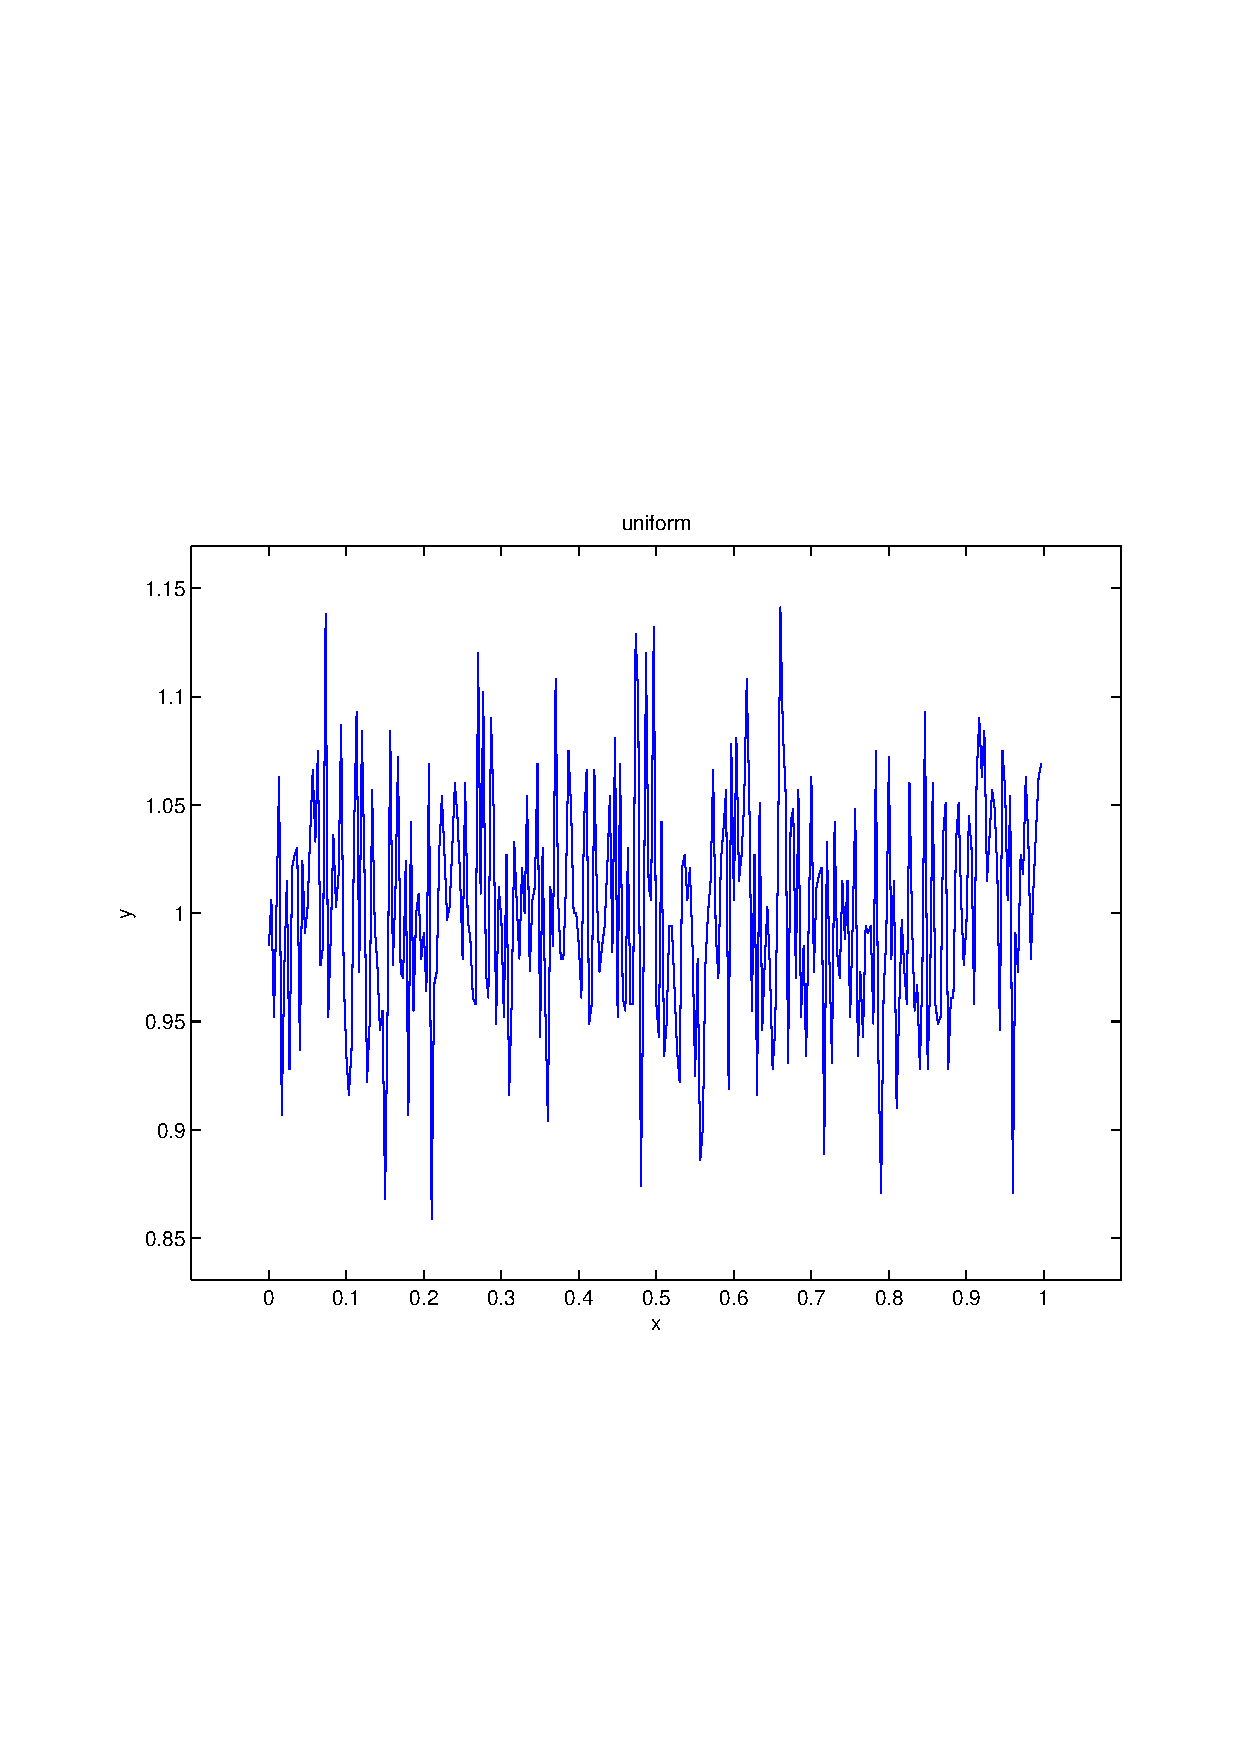
\includegraphics[width=5cm,height=5cm]{uniform.pdf}

cauchy \begin{tabular}{|c|c|c|c|}  mean & variance & skewness & kurtosis \\  \hline
$\mu_1 = +0.44288$ & $\mu_2 = +0.05341$ & $\mu_3 = +0.63935$ & $\mu_4 =+3.28094$ \\
\end{tabular}

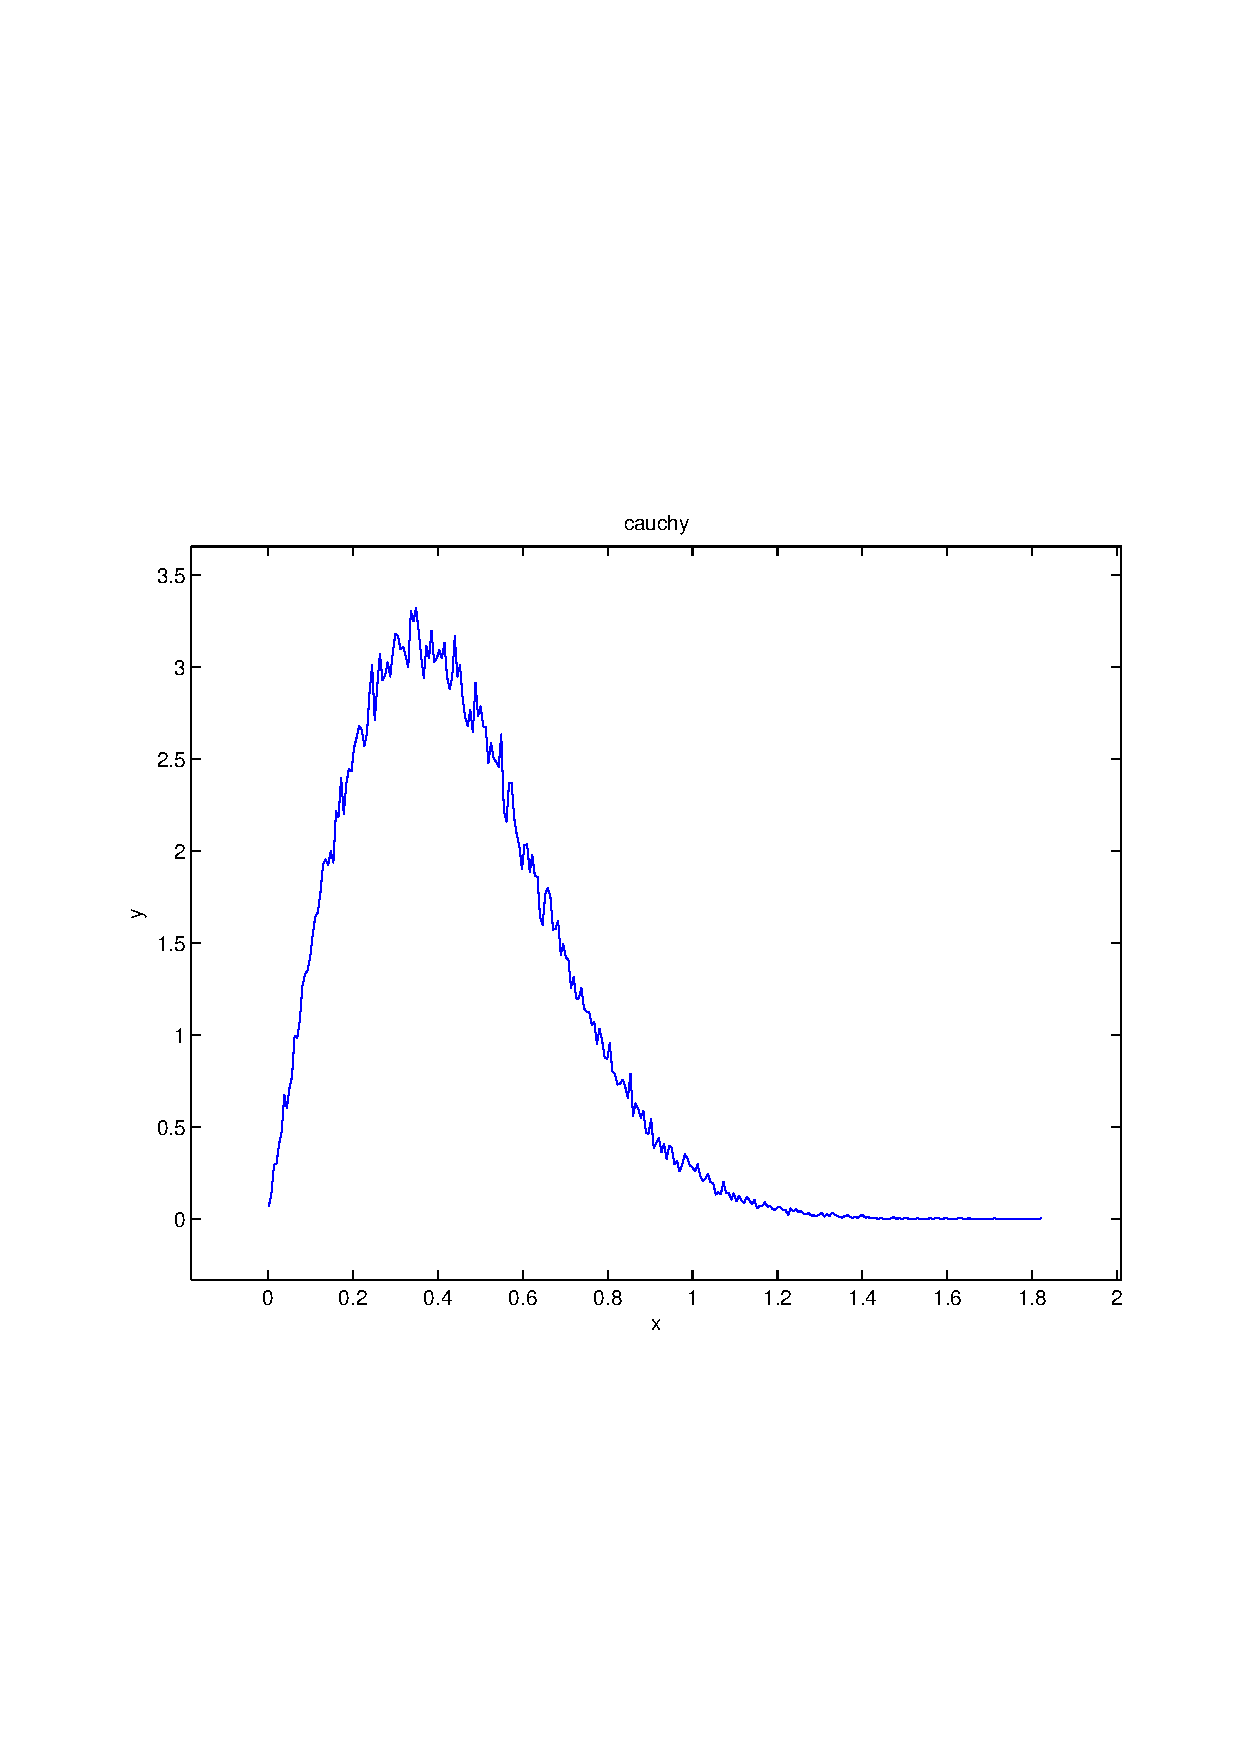
\includegraphics[width=5cm,height=5cm]{cauchy.pdf}

exponential \begin{tabular}{|c|c|c|c|}  mean & variance & skewness & kurtosis \\  \hline
$\mu_1 = +1.99647$ & $\mu_2 = +3.99339$ & $\mu_3 = +2.03097$ & $\mu_4 =+9.30842$ \\
\end{tabular}

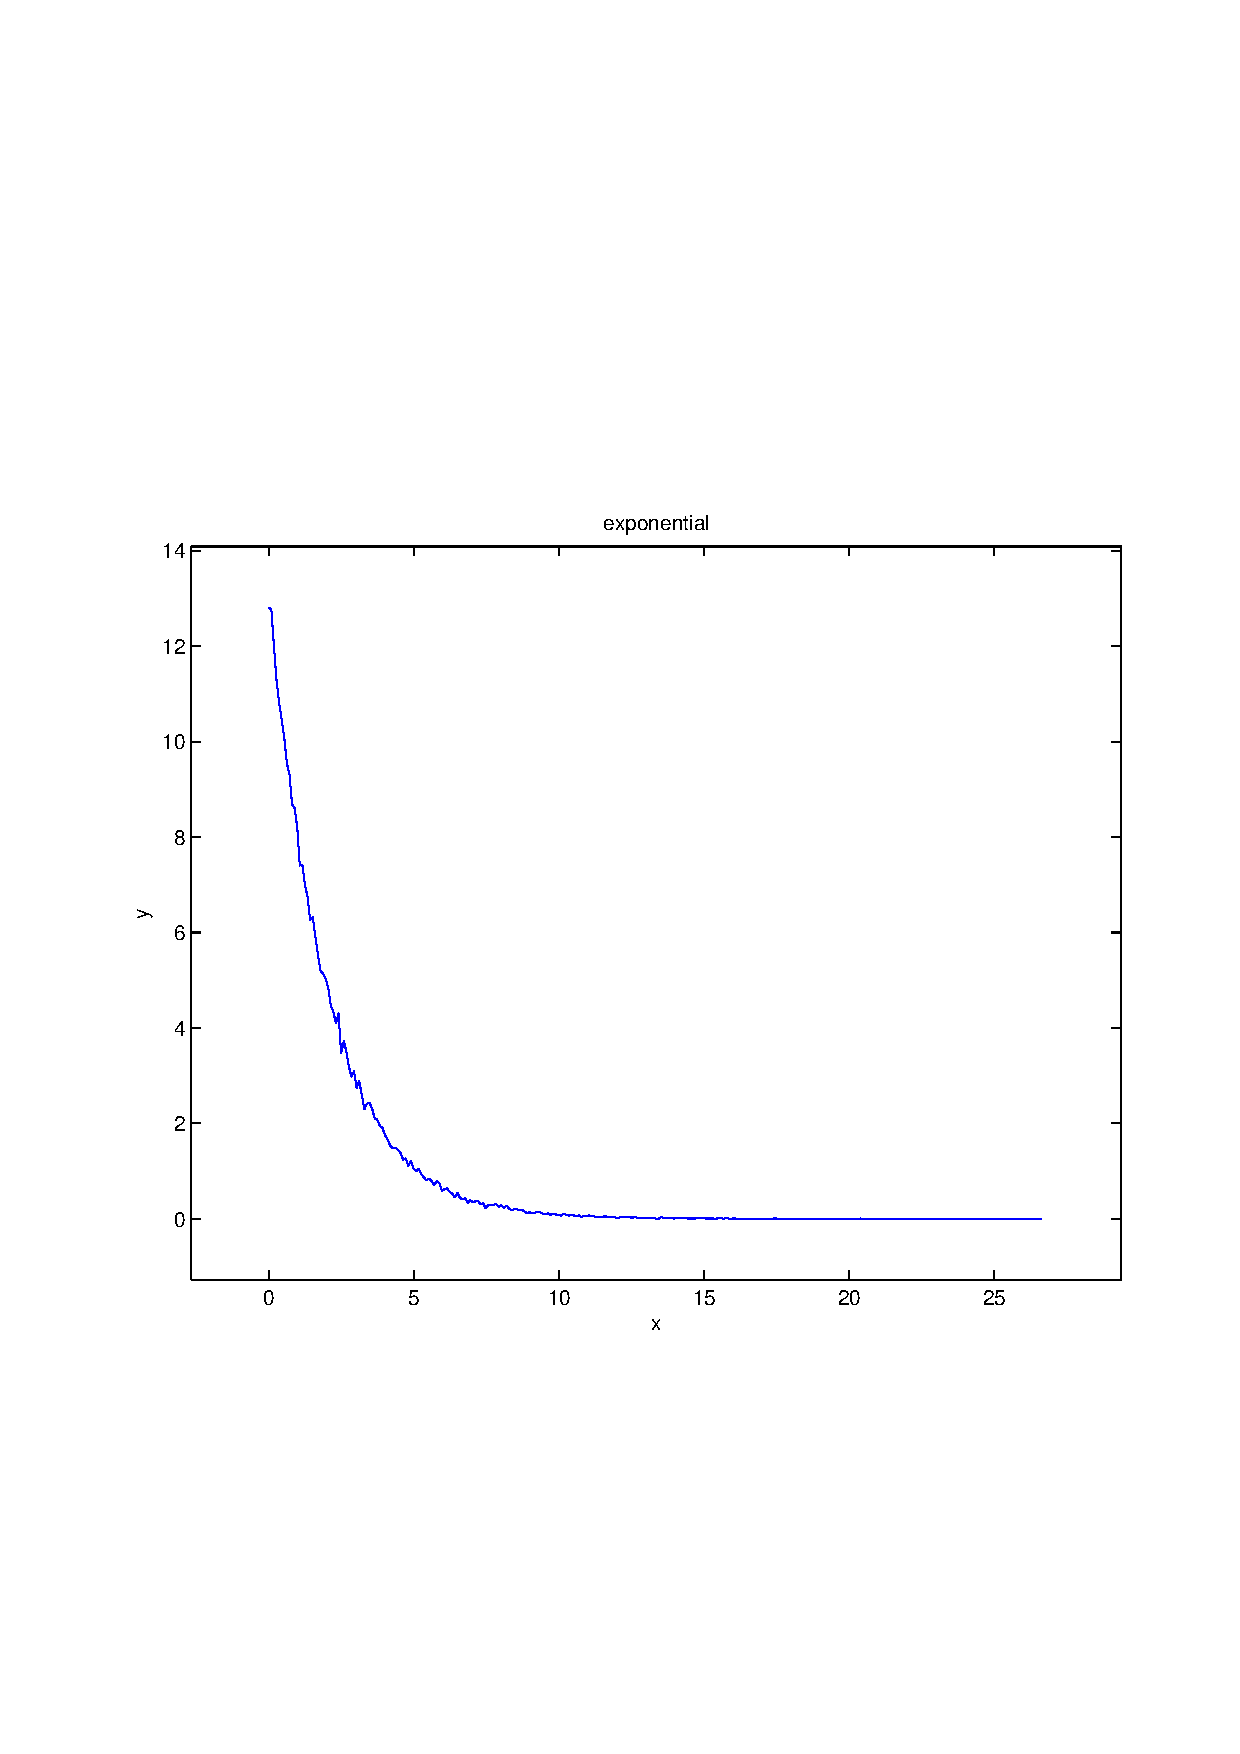
\includegraphics[width=5cm,height=5cm]{exponential.pdf}

\newpage
gamma \begin{tabular}{|c|c|c|c|}  mean & variance & skewness & kurtosis \\  \hline
$\mu_1 = +1.90441$ & $\mu_2 = +1.91502$ & $\mu_3 = +1.45471$ & $\mu_4 =+6.16292$ \\
\end{tabular}

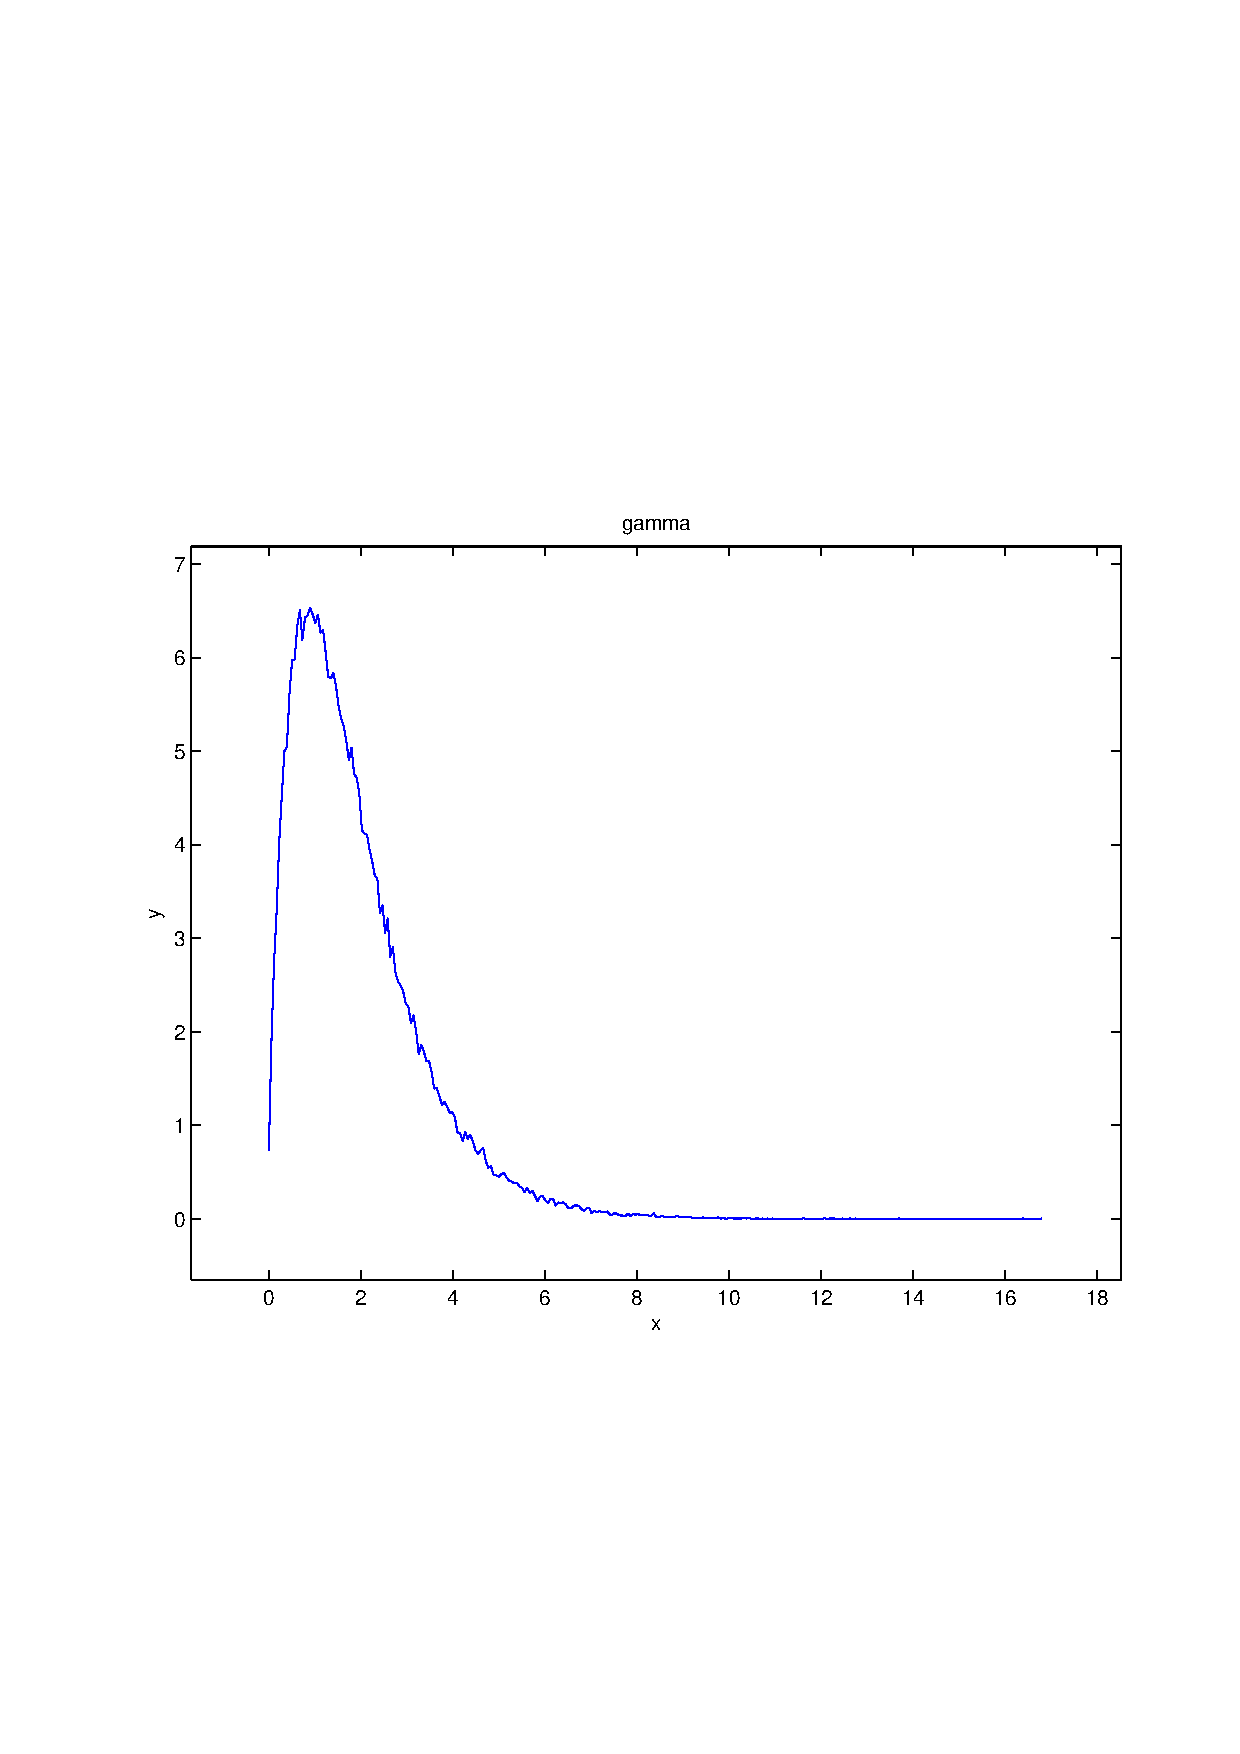
\includegraphics[width=5cm,height=5cm]{gamma.pdf}

GIG \begin{tabular}{|c|c|c|c|}  mean & variance & skewness & kurtosis \\  \hline
$\mu_1 = +0.81945$ & $\mu_2 = +12.08660$ & $\mu_3 = +14.79695$ & $\mu_4 =+289.06232$ \\
\end{tabular}

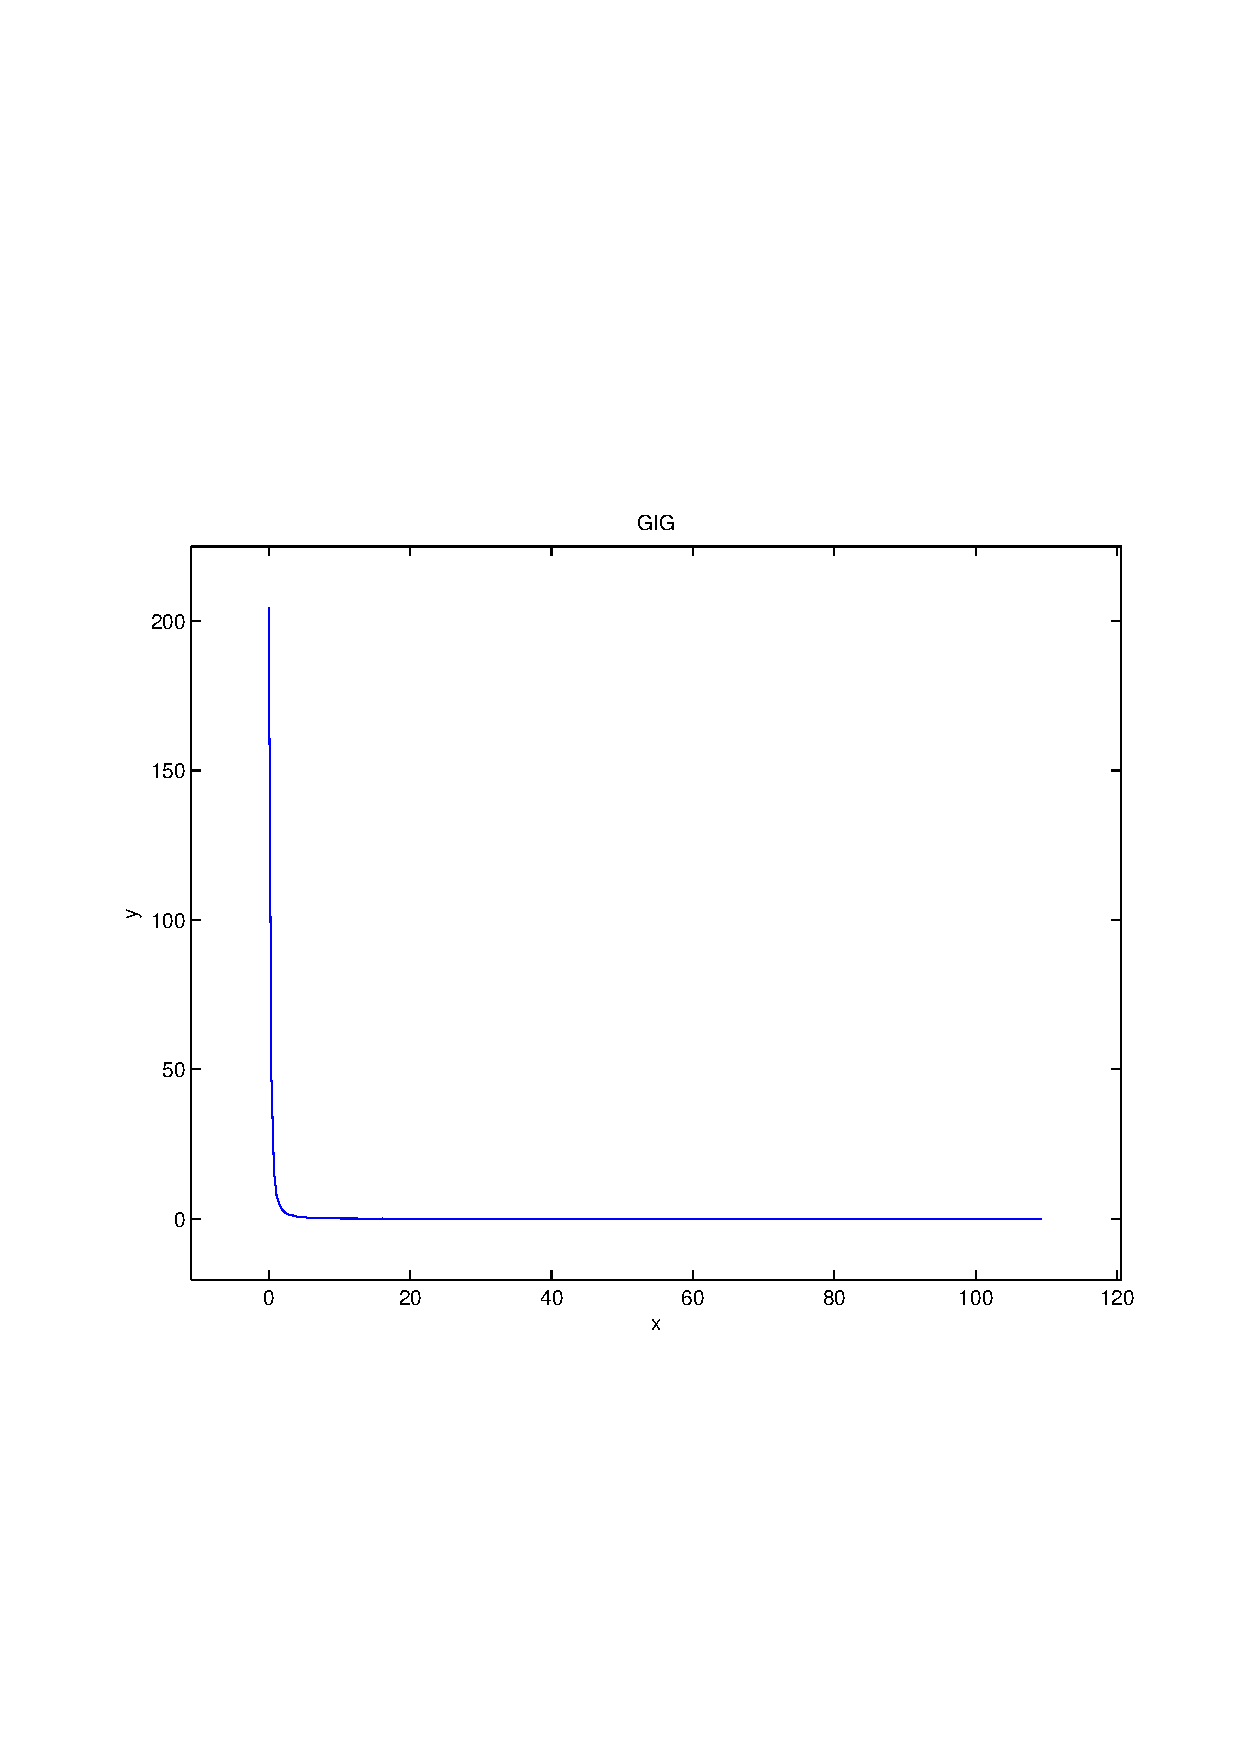
\includegraphics[width=5cm,height=5cm]{GIG.pdf}

normal-box-muller \begin{tabular}{|c|c|c|c|}  mean & variance & skewness & kurtosis \\  \hline
$\mu_1 = +0.00080$ & $\mu_2 = +1.00636$ & $\mu_3 = +0.00747$ & $\mu_4 =+2.99971$ \\
\end{tabular}

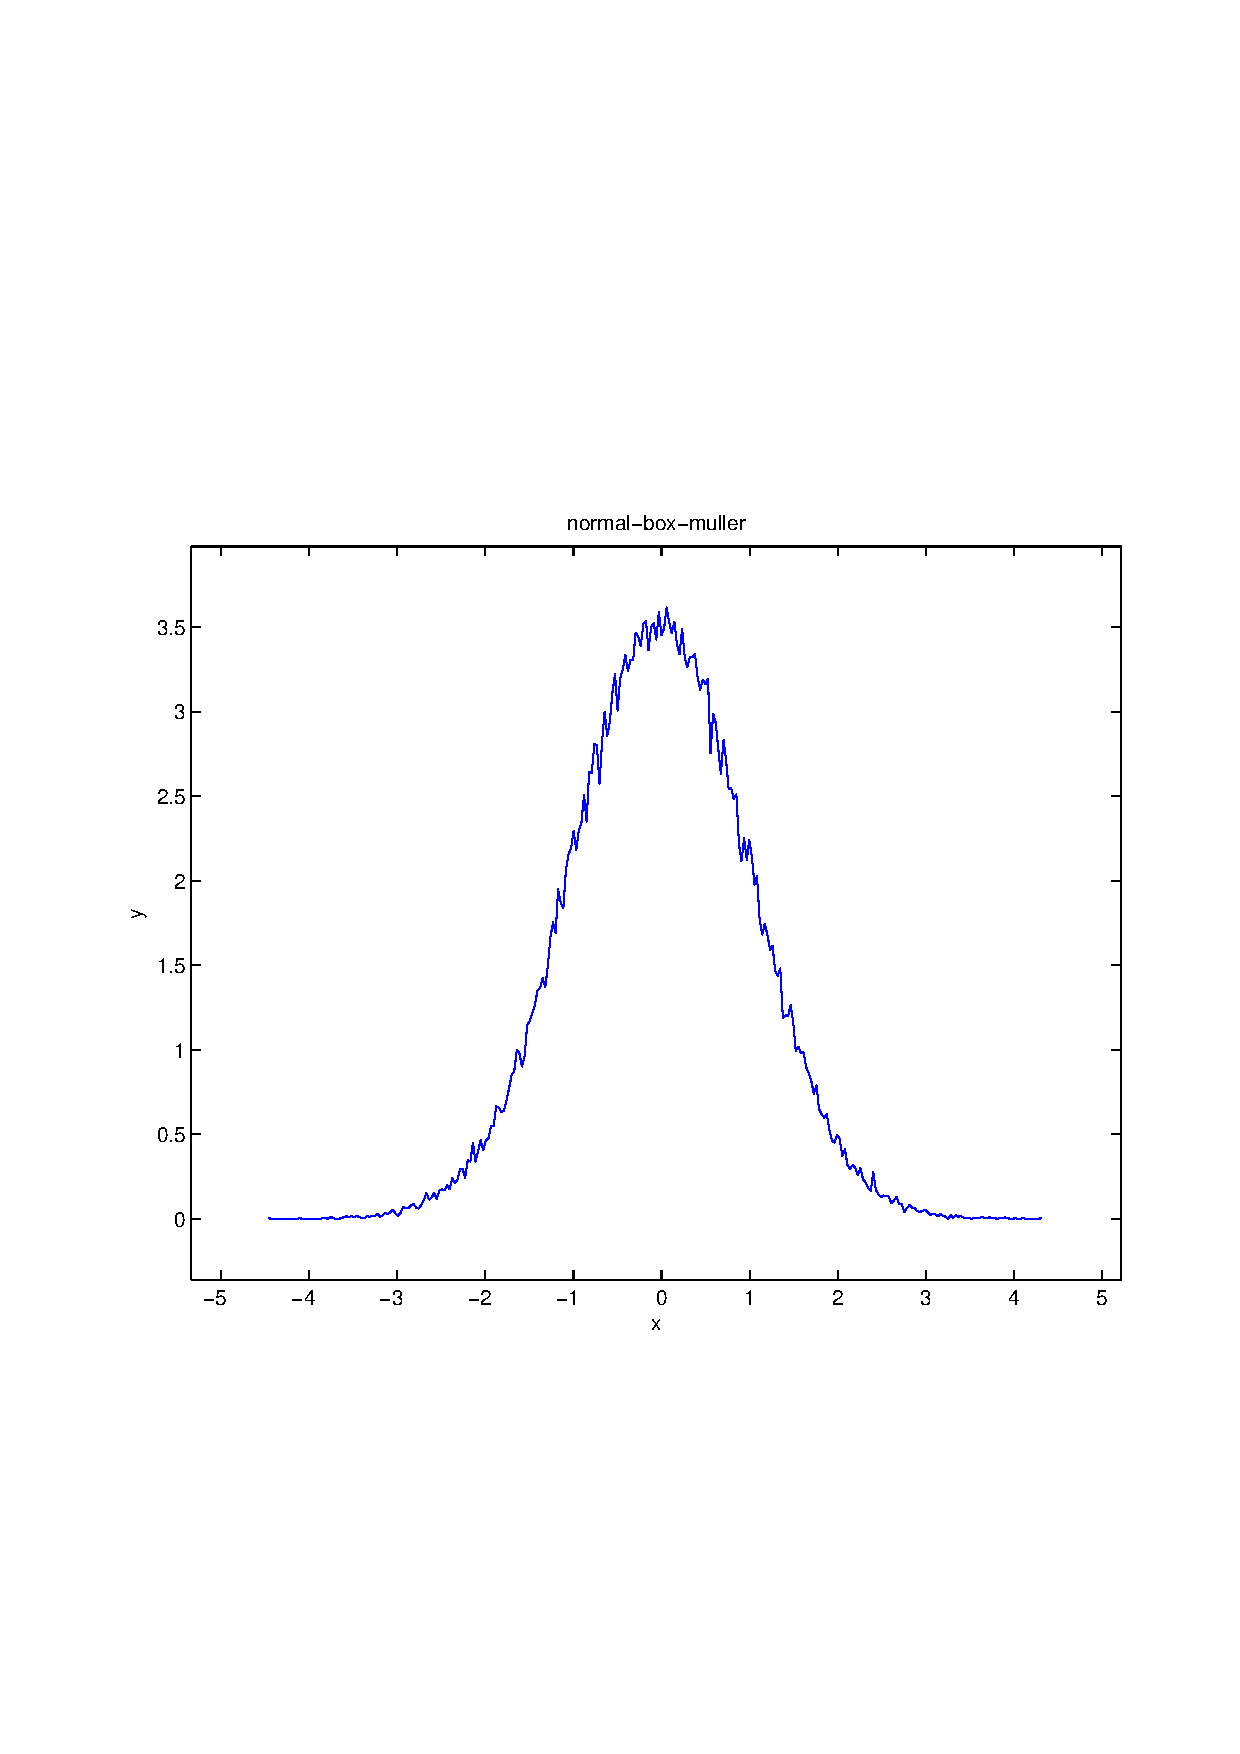
\includegraphics[width=5cm,height=5cm]{normal-box-muller.pdf}

\newpage
normal-inverse-approximation \begin{tabular}{|c|c|c|c|}  mean & variance & skewness & kurtosis \\  \hline
$\mu_1 = +0.00230$ & $\mu_2 = +1.00486$ & $\mu_3 = +0.01163$ & $\mu_4 =+2.99254$ \\
\end{tabular}

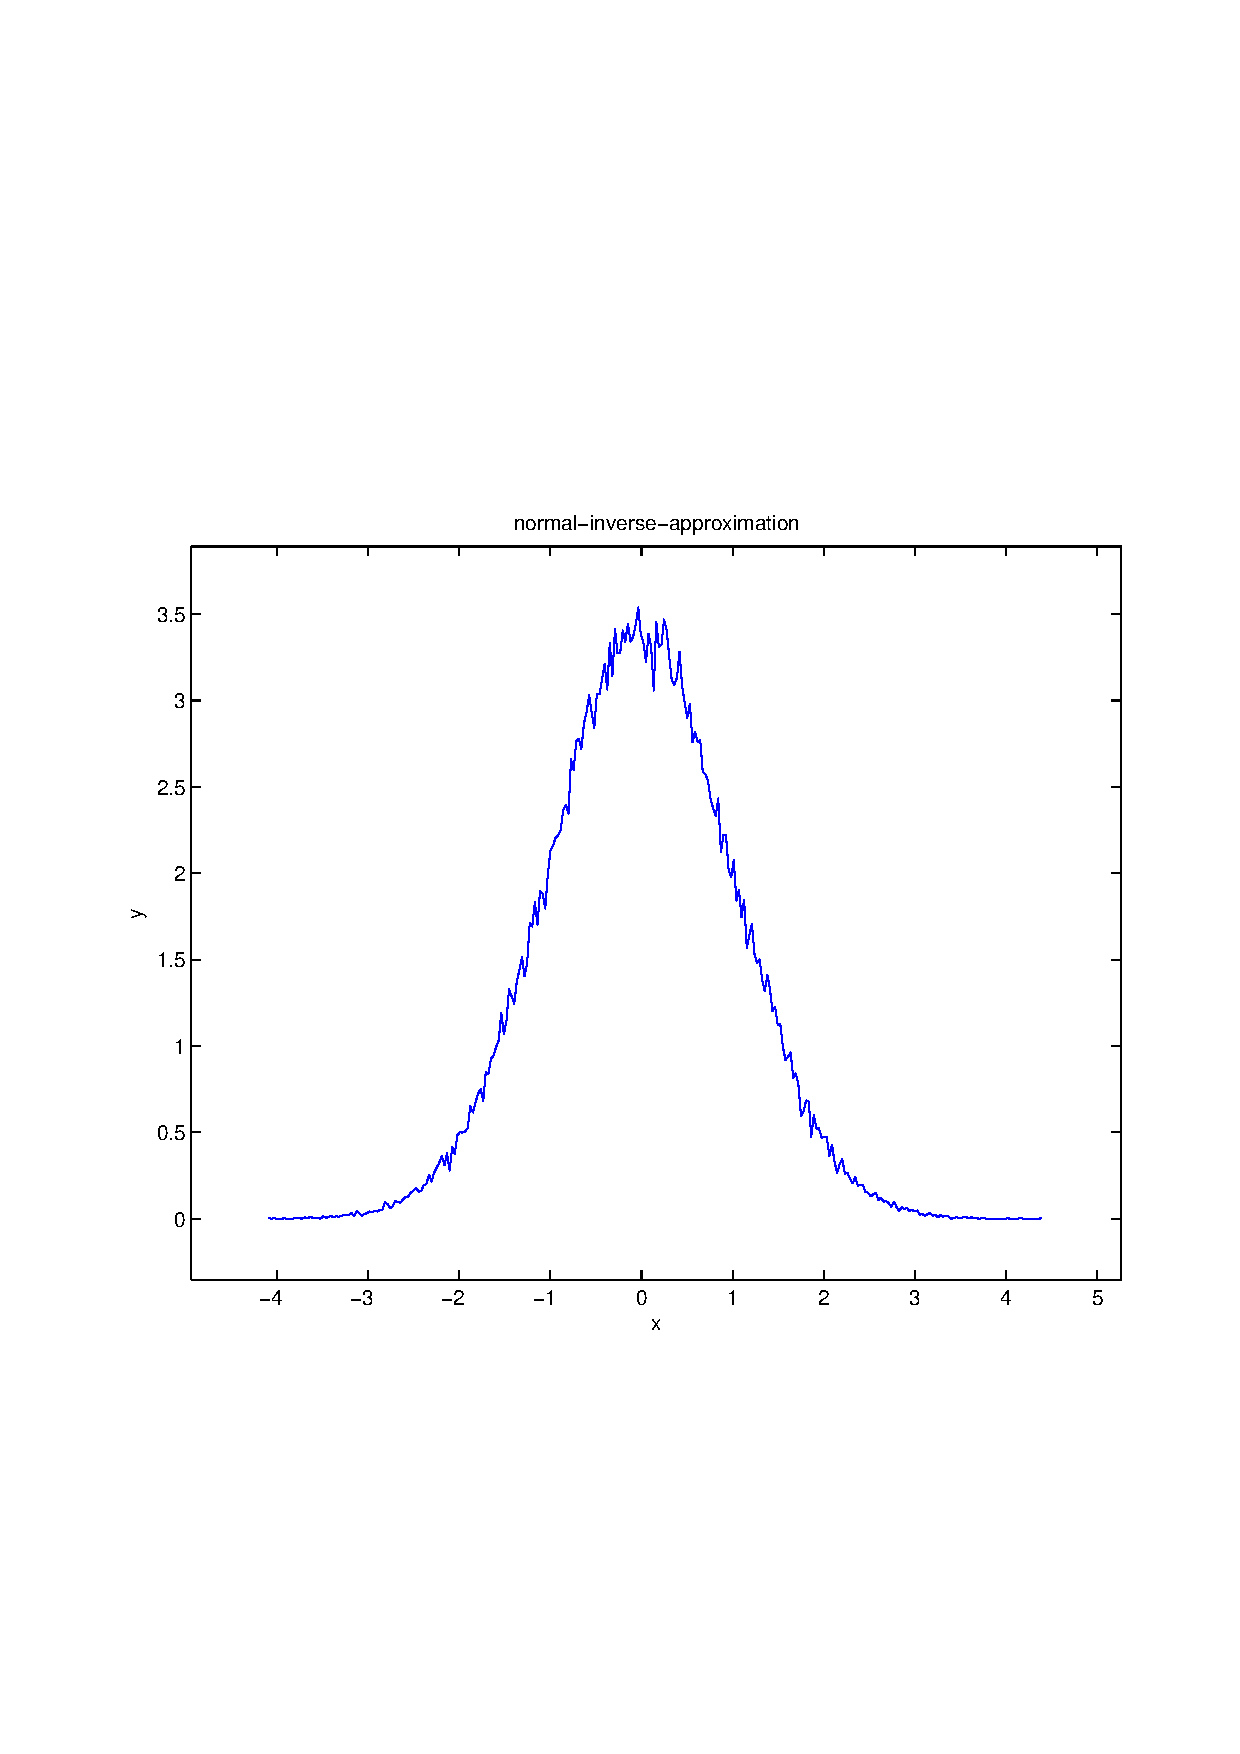
\includegraphics[width=5cm,height=5cm]{normal-inverse-approximation.pdf}

pareto \begin{tabular}{|c|c|c|c|}  mean & variance & skewness & kurtosis \\  \hline
$\mu_1 = +3184578.26493$ & $\mu_2 = +888468246174112900.00000$ & $\mu_3 = +315.36997$ & $\mu_4 =+99629.09819$ \\
\end{tabular}

\includegraphics[width=5cm,height=5cm]{pareto.pdf}

poisson \begin{tabular}{|c|c|c|c|}  mean & variance & skewness & kurtosis \\  \hline
$\mu_1 = +1.10678$ & $\mu_2 = +0.13224$ & $\mu_3 = +3.89832$ & $\mu_4 =+20.82215$ \\
\end{tabular}

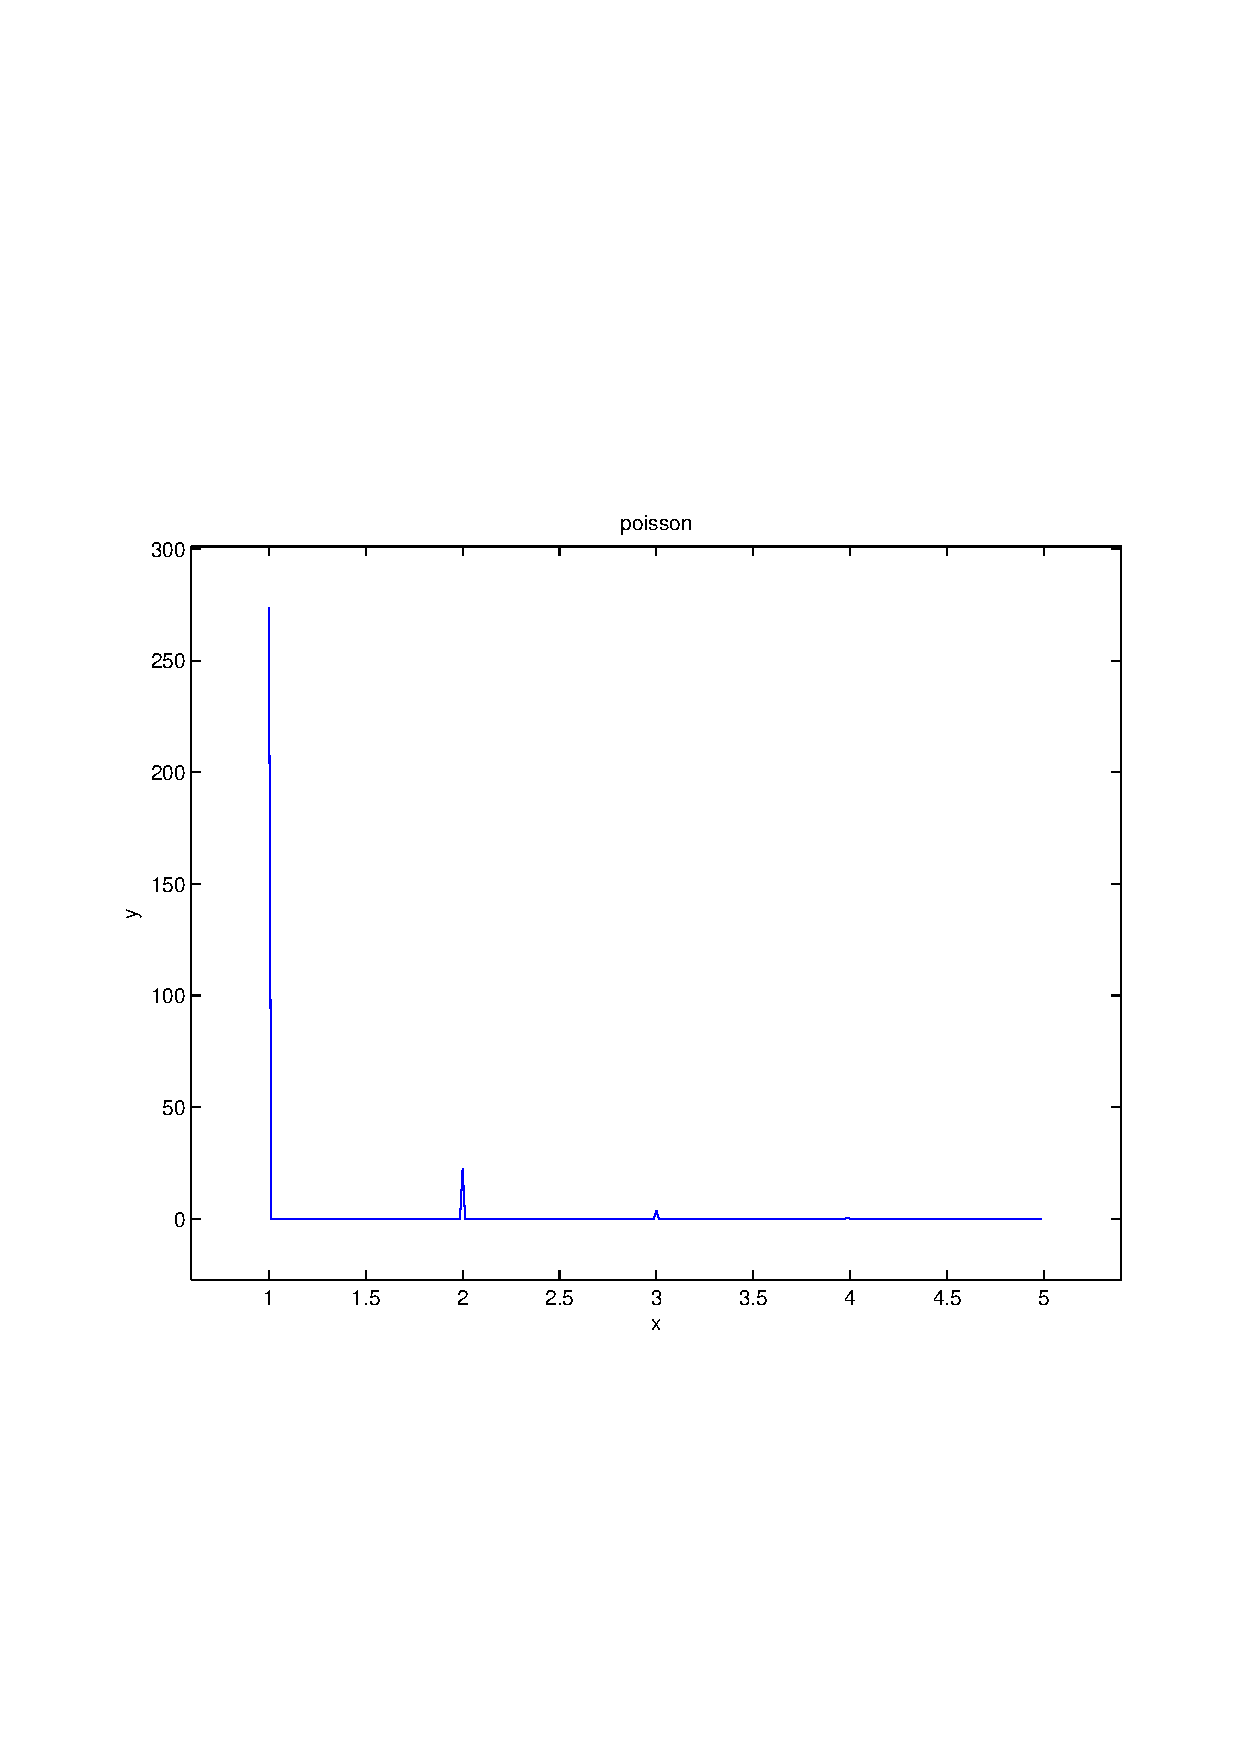
\includegraphics[width=5cm,height=5cm]{poisson.pdf}

\newpage
beta \begin{tabular}{|c|c|c|c|}  mean & variance & skewness & kurtosis \\  \hline
$\mu_1 = +0.33336$ & $\mu_2 = +0.12704$ & $\mu_3 = +0.68068$ & $\mu_4 =+1.90989$ \\
\end{tabular}

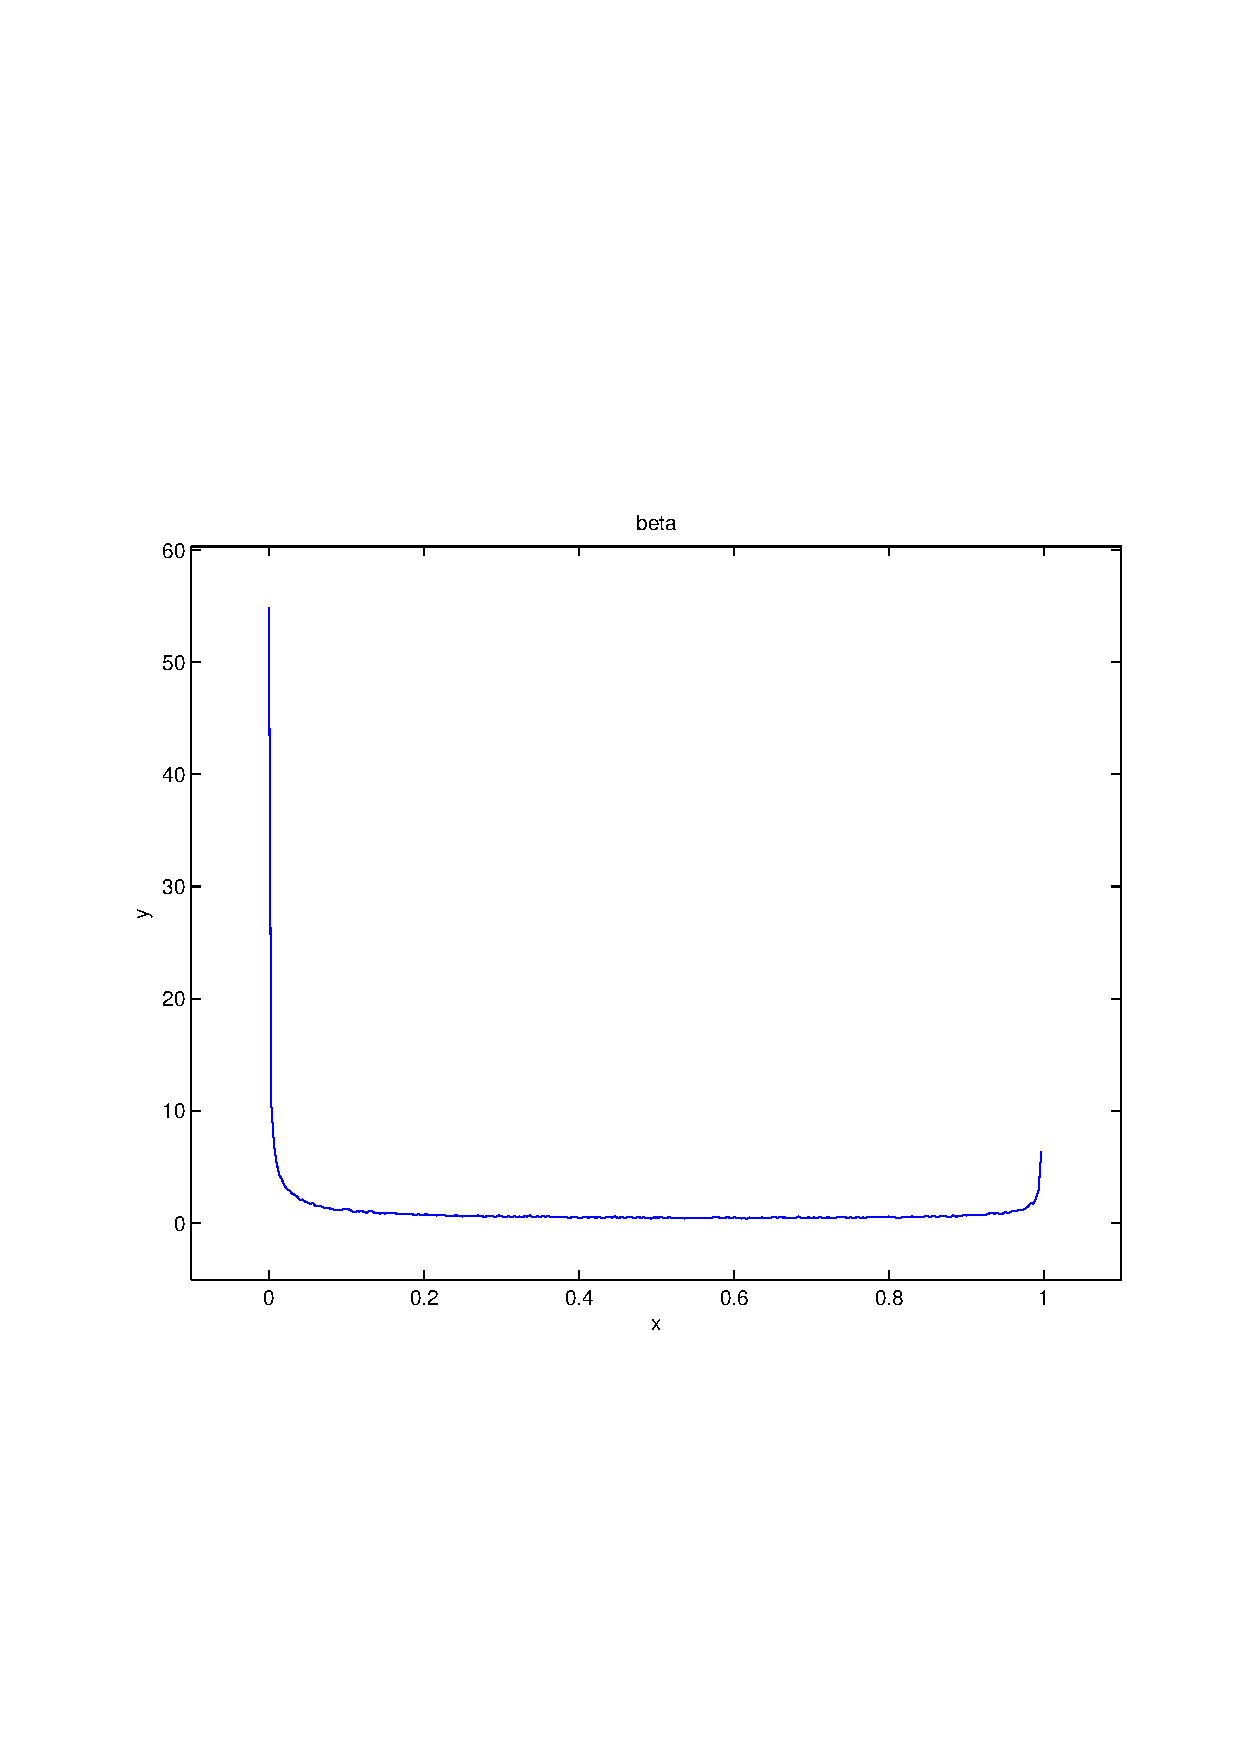
\includegraphics[width=5cm,height=5cm]{beta.pdf}

QueryPerformanceCounter  =  +26.16322
\subsubsection{Multiclass Support Vector Machine }
\begin{itemize}
\item Number or training points = 1024
\item Feature dimension = 3
\item Number or classes = 3
\end{itemize}
{The mean vectors of the 3 classes}

$\mu_1 = \left(
\begin{array}{
ccc}
+1.90000 & +0.10000 & +0.10000 \\
\end{array}
\right)$ \newline 

$\mu_2 = \left(
\begin{array}{
ccc}
+0.10000 & +1.90000 & +0.10000 \\
\end{array}
\right)$ \newline 

$\mu_3 = \left(
\begin{array}{
ccc}
+0.00000 & +0.00000 & +1.90000 \\
\end{array}
\right)$ \newline 

A random SPD covairance matrix is generated for each of the classes.\newline

$\rho_1 = \left(
\begin{array}{
ccc}
+2.804 & +0.327 & -0.396 \\
+0.327 & +3.524 & +0.124 \\
-0.396 & +0.124 & +2.877 \\
\end{array}
\right)$ \newline 

$\rho_2 = \left(
\begin{array}{
ccc}
+2.893 & -0.395 & -0.345 \\
-0.395 & +2.584 & -0.282 \\
-0.345 & -0.282 & +2.181 \\
\end{array}
\right)$ \newline 

$\rho_3 = \left(
\begin{array}{
ccc}
+1.874 & +0.430 & +0.079 \\
+0.430 & +1.814 & -0.139 \\
+0.079 & -0.139 & +3.658 \\
\end{array}
\right)$ \newline 

Verify $L_1$ condition number of covariance. The diagonal entries of the matrix have the form $(0.5 + U(0,1) )*dim(Dom(Cov))$
The lower-diagonal entries take the form $U(0,1) - 0.5$. 
The $L_1$ condition numbers are :
\begin{itemize}
\item +1.814
\item +2.195
\item +2.891
\end{itemize}
\includegraphics[width=10.0cm,height=10.0cm]{rv1_corr.pdf}

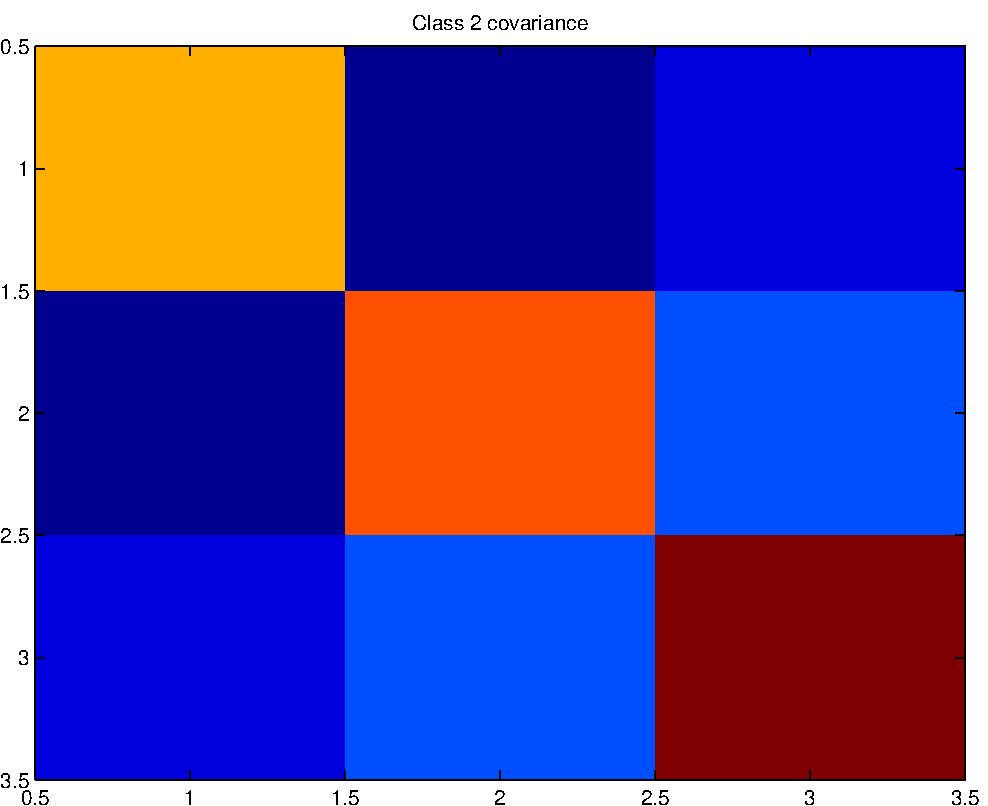
\includegraphics[width=10.0cm,height=10.0cm]{rv2_corr.pdf}

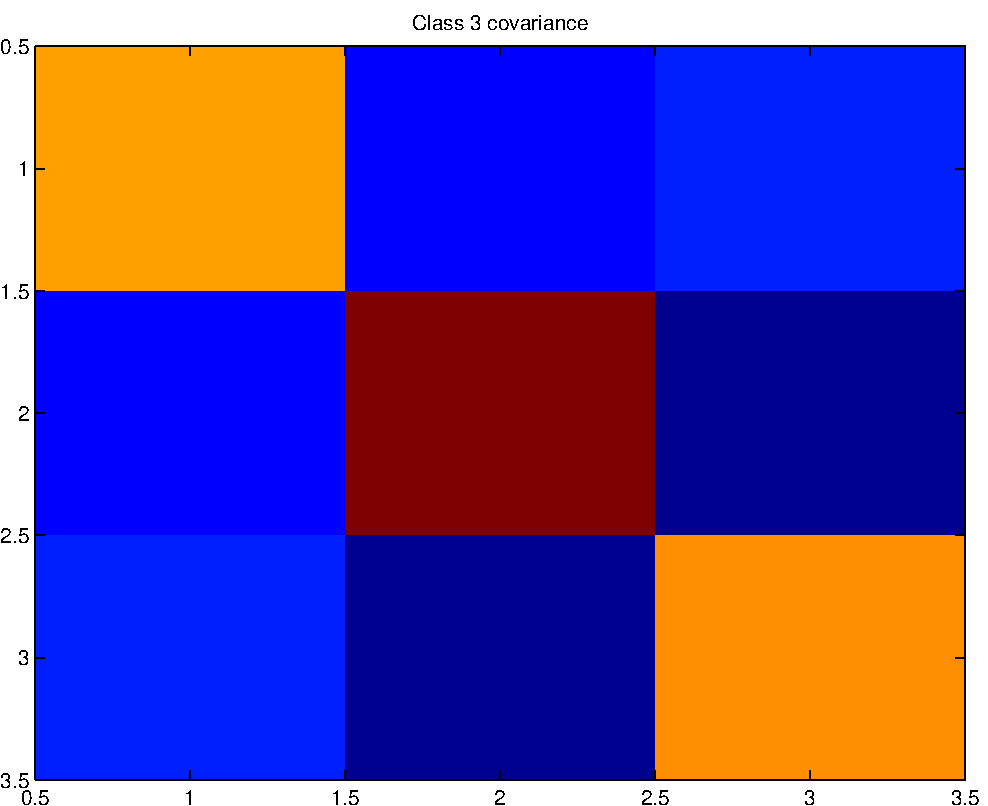
\includegraphics[width=10.0cm,height=10.0cm]{rv3_corr.pdf}

